%% =========================================================================
%% main.tex — Original Research Article for the Semantic Web Journal (Sage)
%% Template: official Sage LaTeX2e class `sagej`.
%% Reference style: Sage Vancouver (numbered), per the SWJ submission guide.
%%   The `sageh` option selects the standard Sage layout; the bibliography is
%%   driven by SageV.bst (Sage Vancouver). See README.md for compilation on
%%   Overleaf (the `sagej` class ships with the Sage demonstration template).
%% =========================================================================
\documentclass[sageh]{sagej}

%% --- Packages -------------------------------------------------------------
\usepackage{moreverb}
\usepackage{booktabs}
\usepackage{amsmath}
\usepackage{url}
\usepackage{graphicx}      %% \includegraphics for the eight figures in figs/
\usepackage{float}         %% [H] places each figure inline, next to its discussion

%% --- Running heads --------------------------------------------------------
\def\volumeyear{2026}

\begin{document}

\runninghead{Anonymous Author(s)}

\title{A Semantic Educational Knowledge Graph with GraphRAG for Programming Feedback: Human-Grounded Criterion Validation of an LLM Judge}

\author{Adrián Bueno Junquero}

\affiliation{Universitat Oberta de Catalunya (UOC), Adjunct Professor, Barcelona, Spain\\
Email: abuenoj@uoc.edu}


%% =========================================================================
%% STRUCTURED ABSTRACT (~200 words): Background / Methods / Results / Conclusions
%% =========================================================================
\begin{abstract}
\textbf{Background:} Knowledge-graph-augmented generation (GraphRAG) is increasingly used to produce pedagogical feedback on student code, yet automated quality verdicts typically rest on an unvalidated ``LLM-as-a-judge'' whose agreement with human educators is rarely measured.
\textbf{Methods:} We build a canonical Educational Knowledge Graph (EKG) for introductory Python (157 concepts) under an OWL~2~RL closure and SHACL constraints, and compare four feedback systems: a base LLM (A), a QLoRA-fine-tuned model (B), GraphRAG (C), and a hybrid (D). Systems are evaluated on a synthetic held-out benchmark (n=50) and on real student code (n=60), with an LLM judge and a blind panel of ten human reviewers (6000 dimension-level ratings).
\textbf{Results:} On synthetic data the hybrid D leads (0.76 category, 0.54 concept), but on real code the ranking inverts (A 0.802 vs.\ D 0.323; Friedman $p=8.1\times10^{-15}$). Inter-judge agreement is weak (Fleiss 0.213); human inter-rater agreement is Fleiss 0.096 yet ICC(2,k) 0.831. Human$\leftrightarrow$judge criterion validity is poor (Pearson 0.203, negative on the popular-explanation dimension; Bland--Altman bias $+0.139$).
\textbf{Conclusions:} The LLM judge is not validated as an absolute scoring instrument, but the averaged human panel is reliable and discriminates the systems.
\end{abstract}

\keywords{knowledge graph, GraphRAG, large language models, criterion validity, inter-annotator agreement, programming education}

\maketitle

%% =========================================================================
\section{Introduction}
%% =========================================================================
Formative assessment is one of the most powerful levers on student learning, but in programming education it does not scale. Cohorts routinely exceed a fifty-to-one student--instructor ratio, while a single piece of individualised feedback on a submission demands fifteen to twenty minutes of expert attention. The classical response (static analysis combined with unit tests) scales effortlessly, yet it verifies behaviour, not understanding. It can report that a test failed without explaining \emph{why} the underlying conceptual model is wrong, and a systematic review of automated feedback for programming exercises found that the overwhelming majority of systems supply only basic diagnostic feedback instead of the conceptual, explanatory feedback that the literature identifies as effective.\cite{keuning2019slr,hattie2007feedback} A structural gap thus opens between feedback that is cheap and feedback that teaches.

Large language models (LLMs) appear to close this gap. They generate fluent, individualised natural-language explanations on demand. Two complementary adaptation techniques dominate practice. Parameter-efficient fine-tuning, exemplified by low-rank adaptation (LoRA) and its quantised variant QLoRA, cheaply specialises a base model to a target feedback register.\cite{hu2021lora,dettmers2023qlora,yang2025lora} Retrieval-augmented generation (RAG) instead conditions the model on external context retrieved at inference time, so that the output is grounded in an authoritative source beyond parametric memory alone.\cite{lewis2020rag} When that external source is a curated knowledge graph (KG), a structure of entities and typed relations enriched with schema and rules\cite{hogan2021kgsurvey}, the resulting GraphRAG pipeline can in principle deliver feedback that is at once pedagogically framed and traceable to explicit domain concepts.\cite{edge2024graphrag,peng2024graphrag,han2025graphrag} In an educational setting the appeal is easy to state. A knowledge graph can encode the prerequisite structure and the documented misconceptions of a curriculum, so that feedback on a faulty recursive function can be grounded in the concept of a base case and its prerequisites.\cite{christou2025ontology,bijl2025skilltrees,qu2024survey}

Yet a direct application of LLMs to this task collides with two well-documented obstacles. The first is hallucination: LLMs confidently produce statements unsupported by any source, a failure mode that is especially damaging in an instructional context where an incorrect explanation actively miseducates.\cite{ji2023hallucination,huang2023hallucination} The second, and the one this article foregrounds, is a problem of \emph{measurement} rather than of generation. Because human evaluation of generated feedback is slow and expensive, the field has largely delegated quality judgement to another LLM acting as an automated rater, the ``LLM-as-a-judge'' paradigm.\cite{zheng2023judging,li2024judges} This is methodologically convenient and increasingly standard, but it rests on an assumption that is seldom tested: that the judge's verdict tracks the verdict a human educator would give. A growing critical literature reports that LLM judges exhibit scoring biases and instability across design choices. In measurement-theoretic terms, such judges are ``neither valid nor reliable'' as instruments.\cite{hackl2023gpt4,yamauchi2025judge,li2025scoringbias,chehbouni2025neither} If reported gains in feedback quality are certified only by such a judge, those gains may reflect the idiosyncrasies of the rater more than genuine pedagogical value. Establishing whether an LLM judge can stand in for human educators is therefore a precondition for trusting any quality claim in this space, and it requires \emph{criterion validation} against actual human ratings, a step that is conspicuously rare.

This article addresses that gap directly. We construct a canonical Educational Knowledge Graph (EKG) for introductory Python, formally closed under the OWL~2~RL profile and constrained by SHACL, and we build a GraphRAG feedback pipeline around it. We then compare four systems in a factorial design---a base LLM (A), a QLoRA-fine-tuned model (B), a GraphRAG variant (C), and a hybrid that combines fine-tuning and graph grounding (D)---using three independent kinds of evidence: objective ground-truth metrics that are immune to any judge, an LLM judge probed for stability across model families, and, as the central methodological contribution, a blind panel of ten human reviewers (seven professional programmers and three university teachers). We evaluate both in distribution, on a synthetic held-out benchmark, and out of distribution, on real student code drawn from a public university corpus, and we report an adverse out-of-distribution result.

\paragraph{Research questions.} Four questions structure the study. \textbf{RQ1:} Can a SHACL-validated, OWL~2~RL-closed Educational Knowledge Graph be constructed that meets explicit structural targets ($\geq$150 concepts) and links verifiably to an open knowledge base? \textbf{RQ2:} Do graph grounding (GraphRAG), fine-tuning (QLoRA), and their combination improve the objective quality of programming feedback over a base LLM, and does any in-distribution advantage transfer to real student code? \textbf{RQ3:} How reliable is an LLM judge of this feedback, both across judge families and against a human panel, that is, what is its criterion validity? \textbf{RQ4:} Is an averaged human panel a reliable and discriminating instrument for this task even when per-rater agreement is low?

\paragraph{Contributions.} We make four contributions. (i) A canonical, openly licensed Educational Knowledge Graph for introductory Python (157 concepts; 1772 asserted triples expanding to 4786 under OWL~2~RL; 30 verified \texttt{skos:exactMatch} links to Wikidata; zero SHACL violations), together with the design rationale for its semantic correctness, in particular the deliberate use of \texttt{skos:exactMatch} rather than \texttt{owl:sameAs}. (ii) A GraphRAG feedback pipeline with an abstract-syntax-tree concept linker and a QLoRA-fine-tuned Spanish feedback generator, and a clean four-way factorial comparison that isolates the contributions of fine-tuning and of graph grounding. (iii) A two-distribution evaluation that documents both an in-distribution win for the augmented systems and an out-of-distribution ranking inversion that we trace to template over-fitting. (iv) Above all, a human-grounded criterion-validity study of the LLM judge. Ten reviewers produced 6000 dimension-level ratings, analysed with Fleiss' $\kappa$, Krippendorff's $\alpha$, the intraclass correlation coefficient and Bland--Altman analysis, which shows that the judge is \emph{not} validated as an absolute instrument while the \emph{averaged} human panel is reliable and discriminates the systems. Our message is methodological. In automated programming-feedback research, an LLM judge cannot be assumed valid, and verdicts should be anchored in objective, judge-immune metrics and in grounding.

%% =========================================================================
\section{Related Work}
%% =========================================================================
Four strands of prior work bear on the contribution: knowledge graphs in programming education, automated feedback generation, RAG and its evaluation, and inter-annotator agreement in automated evaluation. We review each before stating the gap the work fills.

\subsection{Knowledge graphs in programming education}
Knowledge graphs have been surveyed extensively as a general technology, with their defining ingredients (entities, typed relations, schema and ontological constraints over RDF) now well consolidated.\cite{hogan2021kgsurvey} In education specifically, recent surveys catalogue applications spanning ontology construction, learner modelling, resource recommendation and knowledge representation, while consistently flagging weak user-facing evaluation and limited cross-domain transfer as recurring limitations.\cite{qu2024survey,wu2024personalized} A complementary line models curricula and competency structures explicitly: ontologies for representing curriculum and learning material,\cite{christou2025ontology} and competency-based ``skill trees'' that encode prerequisite orderings in a form directly alignable with a concept graph.\cite{bijl2025skilltrees} LLM-assisted construction of such graphs is itself now an active survey topic, reflecting interest in populating domain graphs from course materials at scale.\cite{bian2025llmkg} For knowledge representation we follow the established RDF/RDFS/OWL/SHACL/SPARQL stack and the SKOS vocabulary for concept hierarchies, building on the standards corpus instead of reinventing it.\cite{w3c-owl2-profiles,w3c-shacl,w3c-skos,w3c-rdf11} Relative to this body of work, our graph is distinguished less by novelty of vocabulary than by being a \emph{validated, reasoning-closed} artefact with explicit structural targets and verified external links, used downstream as the retrieval substrate for feedback generation.

\subsection{Automated and LLM-based programming feedback}
Large language models have accelerated the move from pass/fail autograding toward rich formative feedback. The systematic review of automated feedback for programming exercises remains the reference characterisation of the gap (most systems give only diagnostic feedback, few explain the underlying concept), and the broader theory of feedback emphasises that effective feedback must address the learner's conceptual model, not merely report correctness.\cite{keuning2019slr,hattie2007feedback} A wave of recent work targets exactly this: cross-disciplinary surveys of LLM-based autograding,\cite{eneye2025autograding} multi-faceted frameworks that produce rich pedagogical feedback instead of verdicts,\cite{sahu2025autograder} systems that combine LLMs with static analysis to generate next-step hints without revealing the full solution,\cite{birillo2024onestep} pedagogical-feedback systems designed for classroom integration,\cite{scholz2025partnering} feedback for teaching code refactoring,\cite{khairnar2025refactoring} and studies of how students actually engage with such generated feedback.\cite{jacobs2025feedback} On the modelling side, surveys of LLMs for code generation and of LLM-plus-formal code verification frame the evaluation problem,\cite{huynh2025codegen,dolcetti2025dual} and fine-tuning LLMs to analyse multiple dimensions of code review is closely aligned with our dimension-structured feedback (error type, concept, explanation, suggestion).\cite{yu2025codereview} Our QLoRA generator builds on this efficient-fine-tuning lineage\cite{hu2021lora,dettmers2023qlora,yang2025lora,jain2023neftune,hui2024qwen25coder} but differs in that we do not take the fine-tuned system's superiority for granted, testing whether it transfers to real student code.

\subsection{RAG, GraphRAG, and their evaluation}
Retrieval-augmented generation originated as a way to ground generation in retrieved evidence and reduce hallucination.\cite{lewis2020rag,ji2023hallucination,huang2023hallucination} GraphRAG extends this to graph-structured sources, and two recent surveys consolidate the area, both stressing that graph data demand graph-specific retrieval instead of reusing a uniform embedding space.\cite{edge2024graphrag,peng2024graphrag,han2025graphrag} Within education, GraphRAG has been combined with dual knowledge-structure graphs for learning-path recommendation,\cite{cheng2025graphrag} and at the intersection with semantic validation, RAG has been used to produce explanations of SHACL violations.\cite{publio2025xpshacl} The evaluation of RAG systems has converged on reference-free, faithfulness-oriented metrics, most prominently RAGAS, which scores the proportion of generated claims supported by the retrieved context and the precision of that context.\cite{es2023ragas} We adopt it to probe grounding. Our use of GraphRAG is unusual in pairing it with a fine-tuned generator and in measuring grounding both with a custom concept-citation metric and with RAGAS-style claim-level faithfulness, surfacing the tension between the two.

\subsection{Inter-annotator agreement and LLM-as-a-judge validity}
The reliability of any rating, human or model, is quantified with established statistics: Fleiss' $\kappa$ for categorical agreement among many raters,\cite{fleiss1971kappa} Krippendorff's $\alpha$ for ordinal reliability,\cite{krippendorff2018content,marzi2024kalpha} the intraclass correlation coefficient for the reliability of averaged ratings,\cite{shrout1979icc,mcgraw1996icc} Bland--Altman analysis for agreement between two measurement methods,\cite{bland1986agreement} and the Landis--Koch bands for interpreting $\kappa$.\cite{landis1977agreement} For comparing several systems over the same items we use the Friedman test with Nemenyi post-hoc comparisons, following Dem\v{s}ar.\cite{demsar2006comparisons} The LLM-as-a-judge paradigm\cite{zheng2023judging,li2024judges} has rapidly become the default for evaluating generated text, but its trustworthiness is increasingly contested: studies measure GPT-4's rating consistency,\cite{hackl2023gpt4} show that design choices materially change reliability,\cite{yamauchi2025judge} quantify scoring bias,\cite{li2025scoringbias} argue from measurement theory that LLM judges fail both validity and reliability,\cite{chehbouni2025neither} and propose remedies such as panels of disjoint judges\cite{verga2024poll} or inferred thinking traces.\cite{zhang2025judge} A formal alternative-annotator test has been proposed to decide statistically whether a model may replace a human rater.\cite{calderon2025alttest} Most of this literature, however, measures judge--judge consistency or judge behaviour in the abstract. Comparatively little measures judge--\emph{human} criterion validity for a concrete generative task with a real human panel.

\subsection{The gap this work fills}
Across these four strands, knowledge graphs for education, LLM feedback systems, and GraphRAG pipelines are evaluated overwhelmingly either by objective proxies or by an LLM judge whose agreement with human educators is asserted but never measured. The critical judge literature, in turn, rarely closes the loop with a domain-specific human panel. Our work fills that gap by quantifying the criterion validity of an LLM judge of programming feedback against a ten-person human panel, with the full apparatus of inter-rater reliability and Bland--Altman agreement, and by anchoring the system comparison in judge-immune objective metrics. The central finding is one the field needs but seldom reports: that the judge is not a valid absolute instrument while the averaged human panel is.

%% =========================================================================
\section{Background}
%% =========================================================================
The approach rests on a handful of formal notions, which we fix here so that the design choices in Section~4 can be stated without ambiguity.

\subsection{RDF, RDFS and knowledge graphs}
The Resource Description Framework (RDF) models data as a directed, labelled graph of triples $(s,p,o)$, where subjects and predicates are internationalised resource identifiers (IRIs), objects may additionally be literals, and blank nodes denote existential resources.\cite{w3c-rdf11,hogan2021kgsurvey} A knowledge graph is, in this setting, a large RDF graph of entities and relations enriched with schema and rules that give it semantics and allow validation.\cite{hogan2021kgsurvey} RDF Schema (RDFS) adds a light vocabulary (\texttt{rdfs:subClassOf}, \texttt{rdfs:sub\-PropertyOf}, \texttt{rdfs:domain}, \texttt{rdfs:range}) whose semantics are completive rather than restrictive: a domain axiom \emph{infers} a type, it does not flag an error. An \emph{Educational Knowledge Graph} (EKG) specialises a knowledge graph to learning concepts, their prerequisite orderings and their documented misconceptions. We model the concept hierarchy with SKOS (\texttt{skos:broader}/\texttt{narrower}/\texttt{related}) and link a subset of concepts to external entities with \texttt{skos:exactMatch}.\cite{w3c-skos}

\subsection{OWL 2 RL inference}
The Web Ontology Language OWL~2 extends RDFS with a far richer vocabulary for expressing formal semantics. Its profiles trade expressivity for tractability. The RL profile is rule-based, amenable to forward-chaining materialisation over arbitrary RDF graphs in the manner of a Datalog engine, and computes a sound (if, outside the profile, incomplete) deductive closure.\cite{w3c-owl2-profiles} Materialising this closure lets a reasoner derive entailed triples (for example transitive prerequisite chains, or class membership propagated through \texttt{rdfs:subClassOf}) without sacrificing decidability or polynomial-time guarantees. A semantically consequential distinction concerns identity: \texttt{owl:sameAs} asserts that two IRIs denote the same resource and licenses substitution in any position, whereas \texttt{skos:exactMatch} records a close conceptual correspondence without such fusion. The choice between them changes what a reasoner infers, a point that drives a design decision in Section~4.

\subsection{SHACL validation}
Because RDFS and OWL operate under the open-world assumption, they detect logical inconsistency but not the structural \emph{incompleteness} of a given graph. The Shapes Constraint Language (SHACL) is the W3C standard that fills this role, validating an RDF data graph against a shapes graph of node and property constraints (cardinalities, datatypes, value ranges and the like) and emitting a validation report whose \texttt{sh:conforms} flag and zero-or-more \texttt{sh:ValidationResult}s localise every violation.\cite{w3c-shacl} SHACL constraints count terms in the graph rather than restrict interpretations, which makes them the appropriate closed-world tool for asserting that an artefact is well formed. Active research extends SHACL from graphs to datasets,\cite{dao2025shaclds} provides common formal foundations for SHACL, ShEx and PG-Schema,\cite{ahmetaj2025foundations} and supports violation exploration and ontology-pitfall detection.\cite{steinparz2026shaclens,choi2025vspo,maillot2025eatyourown}

\subsection{SPARQL}
SPARQL is the W3C query language for RDF. Its basic graph patterns match sets of triple patterns with variables, and its property paths express reachability over paths of arbitrary length, a graph-native capability with no direct SQL analogue.\cite{w3c-sparql11,ducharme2013sparql} We use \texttt{SELECT} queries to verify structural properties of the EKG, \texttt{CONSTRUCT} to materialise transitive prerequisites, and a federated \texttt{SERVICE} query against Wikidata to corroborate external links. The contrast between query evaluation with and without OWL~2~RL inference is itself an evaluation instrument.

\subsection{RAG and GraphRAG}
Retrieval-augmented generation conditions an LLM on context retrieved at inference time, decoupling the knowledge the model uses from the knowledge it memorised and thereby reducing hallucination.\cite{lewis2020rag} GraphRAG retrieves a subgraph rather than a flat passage, exploiting the relational structure of a knowledge graph so that the injected context carries prerequisites and related concepts, not just isolated facts.\cite{edge2024graphrag,peng2024graphrag} Faithfulness of the generated text to the retrieved context is measured by reference-free metrics in the RAGAS family: claim-level faithfulness (the fraction of atomic assertions the context supports) and context precision (the fraction of retrieved items relevant to the question).\cite{es2023ragas}

\subsection{QLoRA and parameter-efficient fine-tuning}
Low-rank adaptation (LoRA) freezes a pretrained model and learns small low-rank update matrices, drastically reducing the number of trainable parameters.\cite{hu2021lora} QLoRA back-propagates through a 4-bit NF4-quantised frozen base model into LoRA adapters, making single-GPU fine-tuning of multi-billion-parameter models feasible without a measurable loss of quality relative to 16-bit tuning.\cite{dettmers2023qlora,yang2025lora} We additionally apply NEFTune, which injects noise into the embedding layer during instruction tuning to improve generalisation.\cite{jain2023neftune} Our base model is a code-specialised instruction-tuned LLM from the Qwen2.5-Coder family.\cite{hui2024qwen25coder}

\subsection{Reliability and agreement statistics}
We use a coherent set of reliability statistics, each measuring a different thing. Fleiss' $\kappa$ summarises categorical agreement among many raters and is interpreted through the Landis--Koch bands.\cite{fleiss1971kappa,landis1977agreement} Krippendorff's $\alpha$ generalises agreement to ordinal data and to missing values, with values below roughly $0.667$ conventionally regarded as too low to draw firm conclusions and negative values indicating systematic disagreement.\cite{krippendorff2018content,marzi2024kalpha} The intraclass correlation coefficient ICC(2,$k$) measures the reliability not of a single rater but of the \emph{average} of a $k$-rater panel under a two-way random-effects, absolute-agreement model. It can be high even when per-rater $\kappa$ is low, because averaging cancels idiosyncratic rater noise, and it is the statistic of choice for reporting the reliability of a human rating panel.\cite{shrout1979icc,mcgraw1996icc,ruan2024divergent} Bland--Altman analysis assesses agreement between two measurement methods through the mean bias and the limits of agreement.\cite{bland1986agreement} For comparing several systems over the same items we use the Friedman test with Nemenyi post-hoc comparisons.\cite{demsar2006comparisons} That ICC(2,$k$) and per-rater $\kappa$ answer different questions is decisive for the results that follow.

%% =========================================================================
\section{Approach}
%% =========================================================================
Four artefacts make up the approach: a canonical Educational Knowledge Graph, a GraphRAG retrieval-and-generation pipeline, a QLoRA fine-tuning protocol for the feedback generator, and a four-system factorial design that isolates each augmentation's effect.

\subsection{Engineering the Educational Knowledge Graph}
The canonical EKG for introductory Python, the project's semantic core, contains \textbf{157} concepts and \textbf{1772} asserted triples. Materialising the OWL~2~RL closure expands the graph to \textbf{4786} triples, adding 3014 entailed triples. The 157 concepts are organised as typed individuals across seven concept subclasses (cross-cutting principles, paradigms, control structures, library modules, data structures, built-in functions and data types), together with 16 topics and 16 documented misconceptions, over a schema of 20 OWL classes, 21 object properties and 7 datatype properties, authored following established ontology-engineering practice for OWL in Prot\'eg\'e.\cite{debellis2021protege} No individual is typed by hand as a \texttt{cfkg:Concepto}. Membership in the concept class is propagated entirely through \texttt{rdfs:subClassOf}, so that the diagnostic query \texttt{?x a cfkg:Concepto} returns \textbf{0} rows without inference and \textbf{157} rows with OWL~2~RL inference. By design, this 0$\rightarrow$157 contrast is the central demonstration that reasoning, not manual assertion, populates the concept class.

A deliberate semantic decision governs the external links. The 30 verified links to the Wikidata open knowledge base\cite{vrandecic2014wikidata} use \texttt{skos:exactMatch}, not \texttt{owl:sameAs}. Had \texttt{owl:sameAs} been used, the OWL~2~RL reasoner would have folded each external Wikidata entity into the concept class, and the inferred count of \texttt{cfkg:Concepto} would have included those 30 foreign entities. By using \texttt{skos:exactMatch}, the correspondence is recorded without identity fusion, so the reasoner keeps the count at exactly the 157 native concepts, the semantically correct outcome for a curated educational vocabulary. We further articulate the concept hierarchy with 19 \texttt{skos:broader}/\texttt{narrower} links and 16 \texttt{skos:related} links.

We validate the graph against a shapes graph of ten SHACL node and property shapes covering, among others, the requirement that every concept belong to a topic, that difficulty values fall within range, and that exercises carry the mandatory metadata. SHACL validation reports \textbf{0} violations on the canonical graph (\texttt{sh:conforms} true) and, as a negative control, \textbf{6} violations on a deliberately malformed graph in which difficulty is out of range and concepts are missing topics, labels and exercise metadata. We further probed the non-trivial inference behaviour with SPARQL: a \texttt{CONSTRUCT} that flattens the transitive prerequisite closure yields 340 triples without inference and 356 with OWL~2~RL, and a federated \texttt{SERVICE} query retrieves Spanish descriptions for the externally linked concepts from the live Wikidata endpoint. Serialised in Turtle, the graph round-trips losslessly through JSON-LD, N-Triples and RDF/XML, and is released under CC~BY~4.0. Figure~\ref{fig:ekg} summarises the layered architecture of the artefact, from the instance level through the schema, reasoning and validation layers to the external Wikidata links.

\begin{figure}[H]
\centering
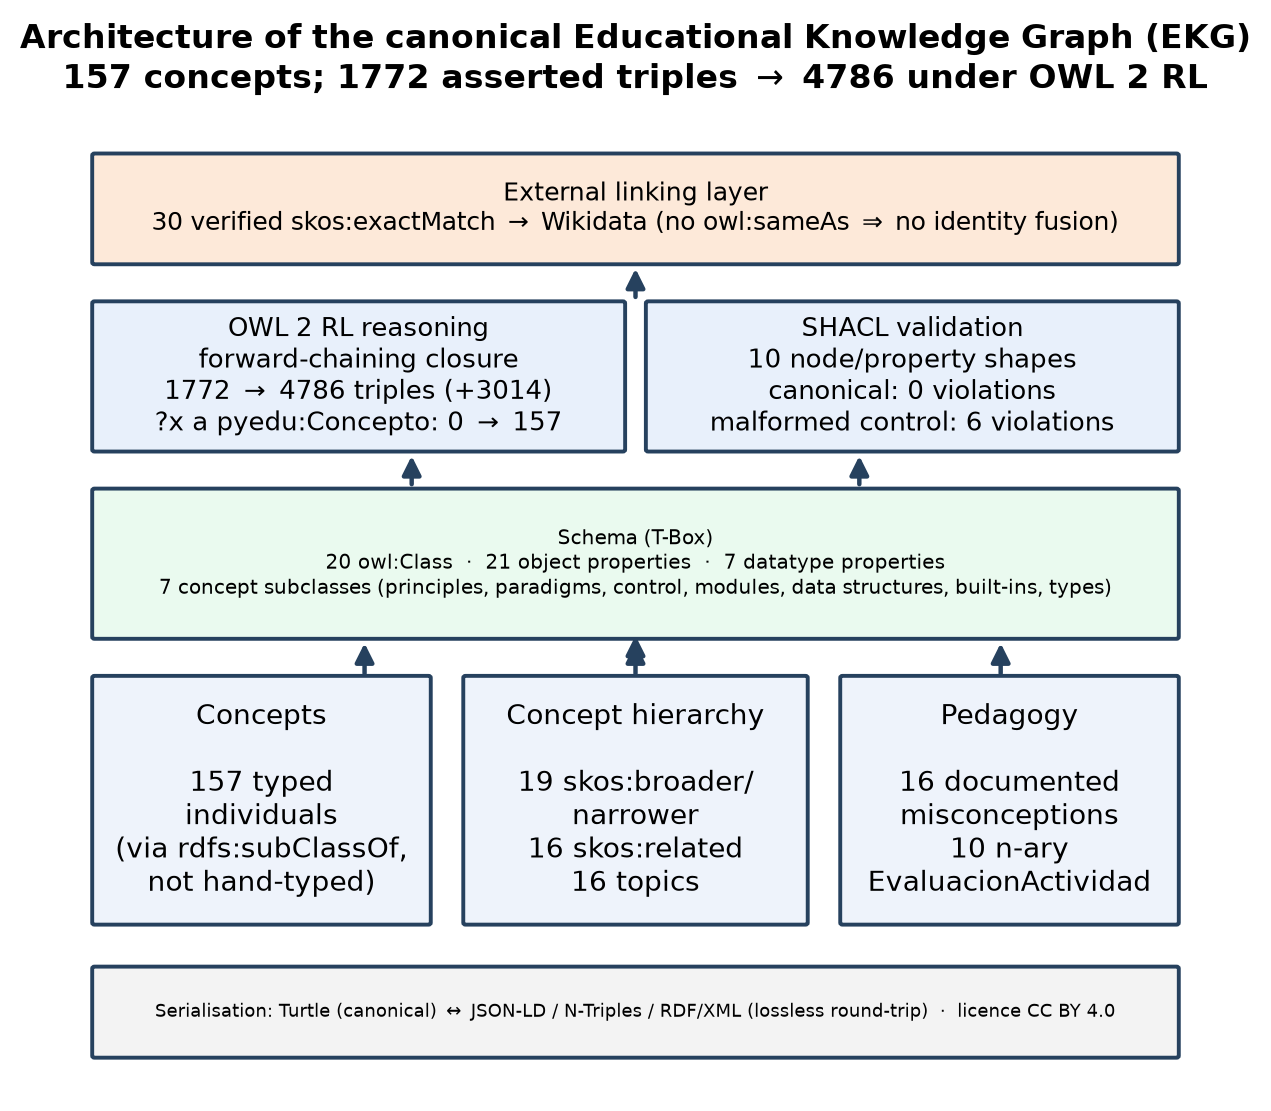
\includegraphics[width=\linewidth]{figs/fig_ekg_architecture_enfix.png}
\caption{Layered architecture of the canonical Educational Knowledge Graph. The instance level holds 157 concepts, 16 topics, 16 misconceptions and 10 n-ary activity-evaluation instances; the schema (T-Box) declares 20 OWL classes, 21 object properties and 7 datatype properties; OWL~2~RL forward-chaining expands the graph from 1772 to 4786 triples and populates \texttt{cfkg:Concepto} from 0 to 157; SHACL reports zero violations on the canonical graph against six on a malformed control; and 30 \texttt{skos:exactMatch} links connect to Wikidata without identity fusion.\label{fig:ekg}}
\end{figure}

\subsection{The GraphRAG pipeline}
Given a student submission, the pipeline produces structured feedback in three stages. First, a concept linker parses the submission's abstract syntax tree (AST) and maps code constructs to EKG concepts. AST-based linking replaces an earlier substring heuristic that produced spurious matches (for instance linking the token \texttt{country} to an exception concept, or an f-string's braces to the dictionary concept). Second, a retriever indexes the 157 concepts by sentence embeddings and returns a top-$k$ subgraph (the matched concepts together with their prerequisites, related concepts and associated misconceptions), fused across the embedding and lexical signals with reciprocal rank fusion. Third, the retrieved subgraph is serialised into the generation prompt, and the generator emits Spanish feedback in a fixed five-part structure: error type, affected concept, popular (lay) explanation, technical explanation and an actionable suggestion. This structure mirrors the dimensions on which the feedback is later scored.

\subsection{The QLoRA fine-tuning protocol}
The fine-tuned generator (System B's adapter, reused by the hybrid D) is a Qwen2.5-Coder-7B-Instruct base\cite{hui2024qwen25coder} adapted with QLoRA: 4-bit NF4 quantisation of the frozen base with low-rank adapters trained on top.\cite{dettmers2023qlora,hu2021lora} The canonical adapter (v3) is regularised with NEFTune ($\alpha=5$)\cite{jain2023neftune} and a LoRA dropout of 0.1, with adapters on all linear modules. Training data are drawn from a synthetic feedback corpus (2625 records) split so that seven structural skeletons are held out of training with zero overlap, an anti-leakage measure motivated below. Regularisation reverses an over-fitting trend present in an unregularised run: held-out evaluation loss falls from 1.051 after the first epoch to \textbf{1.028} after the second (against an unregularised run that rose to 1.410 by the third epoch), and held-out mean token accuracy reaches \textbf{0.842}. The second-epoch checkpoint is selected as the canonical adapter (Figure~\ref{fig:loss}). A preference-alignment variant (ORPO, reference-free, $\beta=0.1$) was additionally trained in a separate, self-contained reconstruction experiment (Linaje~B, distinct from the canonical A/B/C/D study above and not to be conflated with it). Its outcome is a recovery-versus-fine-tuning ablation reported in Section~7.

\begin{figure}[H]
\centering
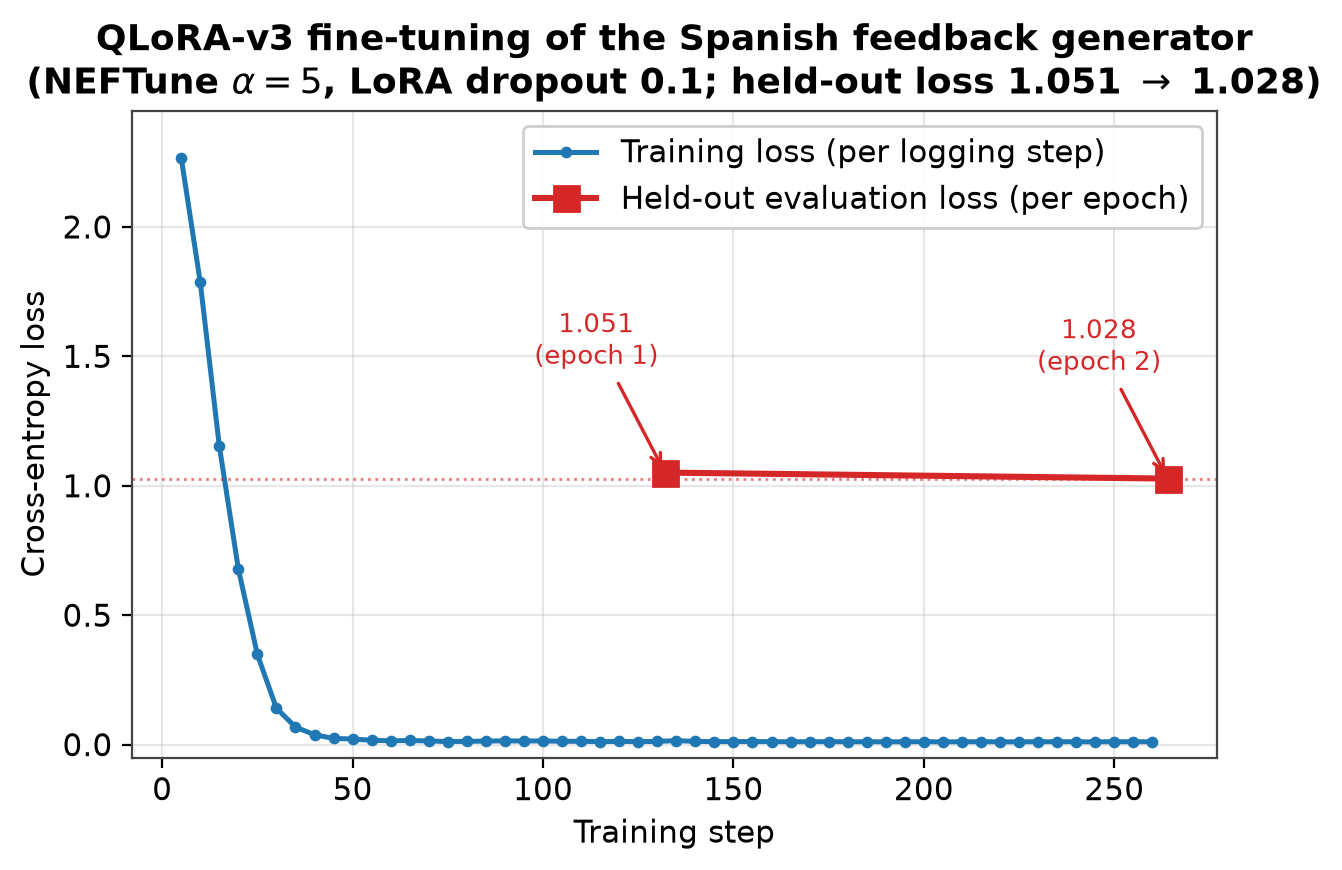
\includegraphics[width=\linewidth]{figs/fig_qlora_loss_enfix.png}
\caption{CFKG-Coder-Adapter-v1 fine-tuning of the Spanish feedback generator (Qwen2.5-Coder-7B-Instruct base; NEFTune $\alpha=5$, LoRA dropout 0.1). The training loss (per logging step) descends steeply, while the held-out evaluation loss falls from 1.051 after the first epoch to 1.028 after the second; the second-epoch checkpoint, where held-out loss is lowest, is selected as canonical.\label{fig:loss}}
\end{figure}

\subsection{The A/B/C/D factorial design}
We compare four systems in a $2\times2$ factorial design crossing fine-tuning with graph grounding. \textbf{A} is the base LLM (\texttt{llama3.1:8b}) with neither augmentation. \textbf{B} is the QLoRA-fine-tuned model without the graph. \textbf{C} is GraphRAG over the base LLM, that is, graph grounding without fine-tuning. \textbf{D} is the hybrid: the fine-tuned model with GraphRAG, combining both augmentations. It isolates the marginal contribution of fine-tuning (A$\rightarrow$B, C$\rightarrow$D), of graph grounding (A$\rightarrow$C, B$\rightarrow$D), and of their combination (A$\rightarrow$D), and is the structure underlying every comparative result below. Figure~\ref{fig:pipeline} depicts the three-stage GraphRAG pipeline and the $2\times2$ factorial layout of the four systems.

\begin{figure}[H]
\centering
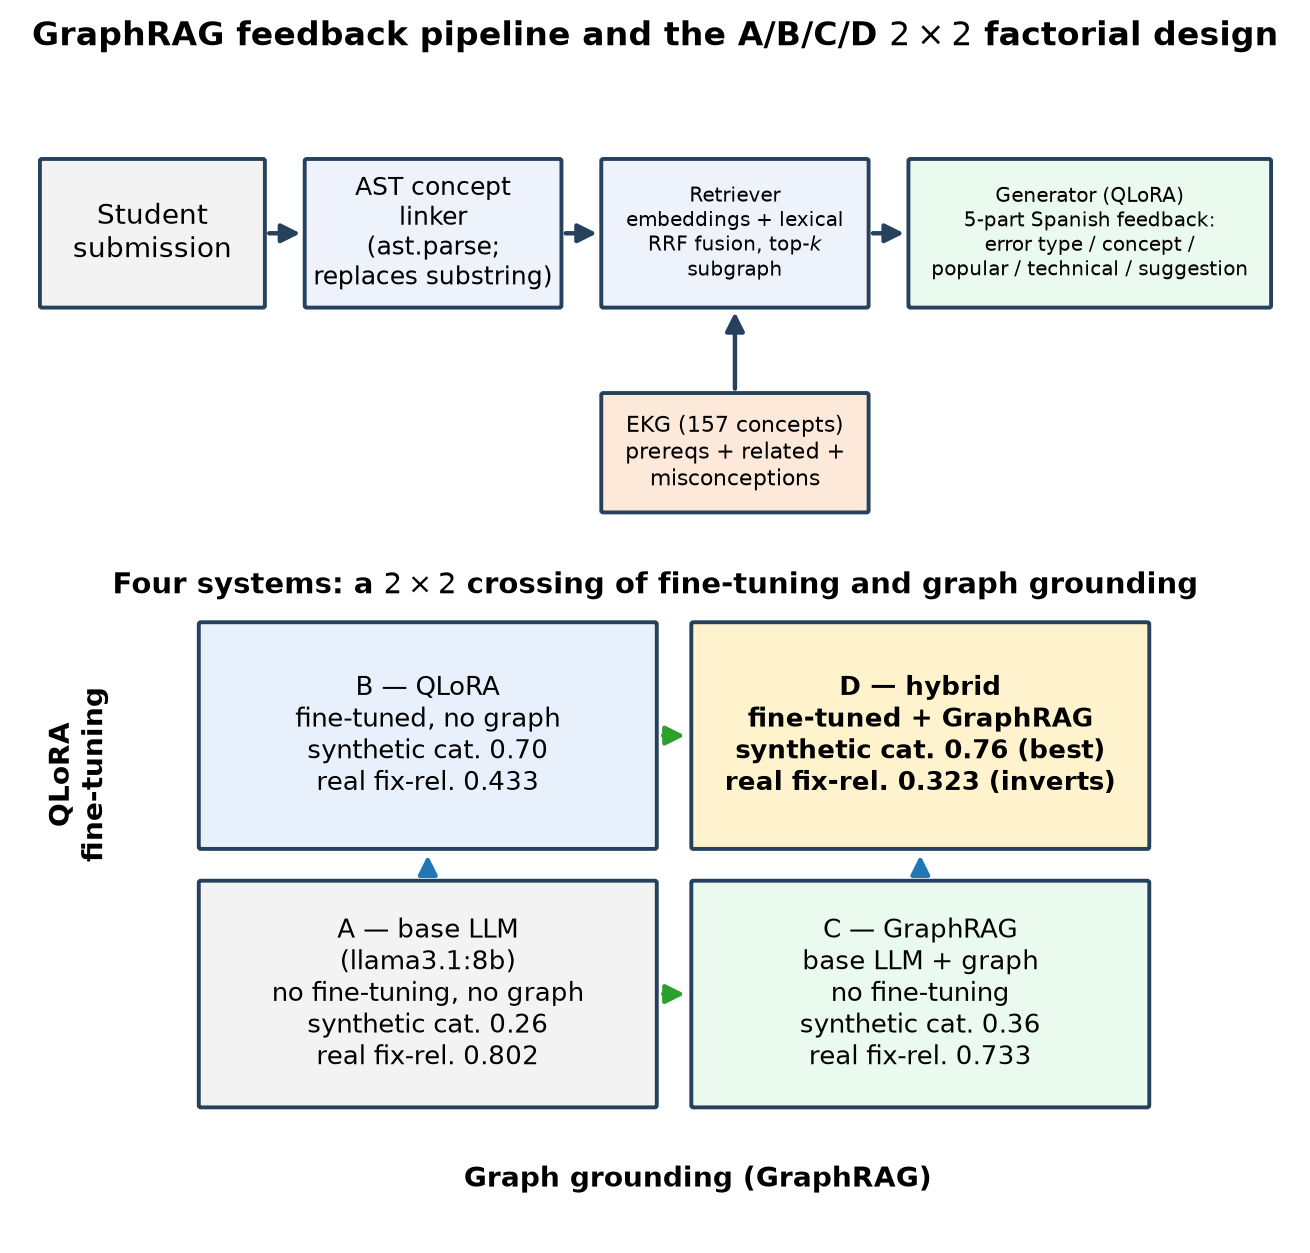
\includegraphics[width=\linewidth]{figs/fig_graphrag_pipeline_enfix.png}
\caption{Top: the GraphRAG feedback pipeline, in which an abstract-syntax-tree concept linker, a reciprocal-rank-fusion retriever over the 157-concept EKG and a QLoRA-fine-tuned generator produce five-part Spanish feedback. Bottom: the four systems as a $2\times2$ crossing of QLoRA fine-tuning (vertical) with graph grounding (horizontal)---base A, fine-tuned B, GraphRAG C and the hybrid D---annotated with the synthetic category accuracy and the real-code fix relevance that invert between the two distributions.\label{fig:pipeline}}
\end{figure}

%% =========================================================================
\section{Experimental Setup}
%% =========================================================================

\subsection{Datasets and their diversity}
We use two evaluation sets, one in distribution and one out of distribution. The \emph{synthetic} held-out benchmark ($n=50$) is drawn from structural skeletons not seen during fine-tuning. For each case an objective ground truth (the intended error category and affected concept) is known, so the principal metrics are anchored to ground truth and independent of any judge. A diversity audit quantifies a key threat to validity in this set: although the underlying synthetic corpus has 53\% unique target strings, semantic diversity is far lower. The mean cosine similarity \emph{within} a skeleton is 0.962, against a global mean of 0.604, so the ``unique'' targets differ largely in variable names within each of the small number of skeletons. Such intra-skeleton homogeneity is the quantified root cause of the over-fitting documented later, and it motivates the second dataset.

The \emph{real} set ($n=60$; 54 unique submissions, with six duplicate identifiers carrying minor double weight) is an out-of-distribution generalisation test drawn from the public Dublin DCU CS1 ``intro\_prog'' repair corpus (\texttt{koutch/intro\_prog}). Here the educator's buggy$\rightarrow$fix diff is the ground truth, and the objective metric \texttt{relevancia\_arreglo} (fix relevance) is the fraction of tokens in the real fix that the feedback references. For safety, code is never executed: only \texttt{ast.parse} and diffing are applied. By breaking the intra-skeleton homogeneity of the synthetic set, this corpus provides the stronger test of generalisation.

\subsection{Models and infrastructure}
Systems A and C use \texttt{llama3.1:8b} as the base LLM, while systems B and D use Qwen2.5-Coder-7B-Instruct with the canonical CFKG-Coder-Adapter-v1 adapter. The LLM judge is \texttt{qwen2.5:32b}. All models run locally for data sovereignty and zero marginal cost, on a single NVIDIA RTX~5090 (32~GB) under Python~3.12. The random seed is fixed at 11 throughout. We note, and control for, the partial within-family overlap between the judge (Qwen) and systems B/D (also Qwen): it is one reason the verdict is anchored in judge-immune objective metrics.

\subsection{Evaluation protocol: objective metrics, LLM judge and human panel}
We combine three kinds of measurement. \emph{Objective} metrics are anchored to ground truth and immune to any judge: category accuracy and concept accuracy on the synthetic set, and fix relevance on the real set. Two further rule-based scores (identification D1 and traceability D5, on a 1--5 scale) are deterministic affine recodings of category and concept accuracy and are reported as alternative scales of the same two axes, not as independent confirmations. \emph{Judge} scores rate three qualitative dimensions (popular explanation, technical explanation and suggestion) on a 1--5 scale with the LLM judge. To probe judge stability, a multi-family panel (Qwen, Llama and Gemma, three providers) re-scored the qualitative dimensions following the panel-of-LLM-evaluators protocol and its caution that nominally distinct judges may not be effectively independent.\cite{verga2024poll,li2024judges} Faithfulness to the retrieved subgraph was measured both with a custom concept-citation grounding metric and with RAGAS-style claim-level faithfulness and context precision.\cite{es2023ragas}

\emph{Human} annotation is the central instrument. Ten reviewers blind-rated the four systems' feedback over the 50 held-out cases on the same three qualitative dimensions, with systems anonymised and shuffled in a self-contained annotation harness. Each reviewer produced 200 rows (50 cases $\times$ 4 systems), each row carrying three Likert scores, for 600 dimension-level scores per reviewer. Across ten reviewers this is 2000 rows and \textbf{6000} dimension-level human ratings, against the judge's 600 cells. The 50 case identifiers are identical across all ten reviewers. Agreement is reported with Fleiss' $\kappa$, Krippendorff's $\alpha$ and ICC(2,$k$); human$\leftrightarrow$judge criterion validity with Pearson and Spearman correlation and Bland--Altman analysis, where the human consensus is the per-cell mean of the ten reviewers.\cite{fleiss1971kappa,krippendorff2018content,shrout1979icc,bland1986agreement}

\subsection{Recruitment of the human panel}
The panel comprises ten volunteers, all with deep Python knowledge, identified only by codes R01--R10 at their explicit request that no names or affiliations be published. It is made up of seven professional programmers (R01, R02, R04, R05, R07, R08, R09) and three university teachers (R03, R06, R10). The programmers span senior backend, fullstack, data, DevOps/SRE, frontend, machine-learning and QA roles with four to nine years of experience; the three teachers are a computer-science lecturer with twelve years teaching introductory programming, a tenured software-engineering professor researching educational software quality, and a university programming instructor with eleven years of teaching experience. The presence of the three domain experts justifies a conservative threshold in the downstream substitution test. Reviewers were informed of the purpose and of the anonymous, aggregate use of their ratings before annotating. The ratings contain no personal data.

%% =========================================================================
\section{Results}
%% =========================================================================

\subsection{The semantic artefact (RQ1)}
The EKG meets its design target. It has \textbf{157} concepts (target $\geq$150) and \textbf{1772} asserted triples expanding to \textbf{4786} under OWL~2~RL (+3014 entailed). The reasoning contrast matches the design: \texttt{?x a cfkg:Concepto} returns 0 rows without inference and 157 with inference, and the \texttt{skos:exactMatch} modelling keeps the inferred concept count at the 157 native concepts instead of absorbing the 30 Wikidata entities. SHACL validation reports \textbf{0} violations on the canonical graph and \textbf{6} on the malformed negative control, and the 30 \texttt{skos:exactMatch} links to Wikidata are individually verified. RQ1 is answered affirmatively: a validated, reasoning-closed, externally linked EKG that meets its structural targets is achievable.

\subsection{Benchmark results in distribution (RQ2)}
On the synthetic held-out benchmark ($n=50$), the hybrid \textbf{D} leads on the objective metrics, with \textbf{0.76} category accuracy and \textbf{0.54} concept accuracy, ahead of B, C and the base A (Table~\ref{tab:n50}). The factorial pattern is informative: fine-tuning (B) most improves error-type classification (category 0.70), graph grounding (C) most improves concept accuracy (0.48) and traceability, and the hybrid D combines both, winning or tying on every dimension. Inferential analysis with the Friedman test and Holm-corrected Wilcoxon post-hoc comparisons confirms that all augmented systems (B, C, D) beat the base A significantly on the objective metrics (for category accuracy, Friedman $p<0.0001$ with a bootstrap 95\% confidence interval for D$-$A of $[+0.36,+0.64]$), but that D's advantage over B is \emph{not} significant at this sample size ($p=0.18$ for category). Augmentation (graph and/or fine-tuning) therefore significantly improves over the base LLM, while the hybrid's superiority over the fine-tuned model alone is numerically present but statistically unconfirmed at $n=50$. A grounding analysis adds nuance to the hybrid's value: D is nearly twice as faithful to the retrieved subgraph as C on the custom concept-citation metric (0.65 vs 0.35) while citing fewer concepts (2.56 vs 5.24 per case), whereas at the level of atomic claims the RAGAS-style faithfulness of C and D is comparable (0.62 vs 0.58) and context precision is identical (0.375), pointing to the retriever rather than the generator as the locus for further improvement.

\begin{table}[t]
\centering
\caption{Synthetic held-out benchmark ($n=50$): objective metrics (category, concept) are anchored to ground truth and judge-independent; qualitative dimensions are LLM-judge scores (1--5). The hybrid D leads or ties throughout.\label{tab:n50}}
\begin{tabular}{@{}lcccc@{}}
\toprule
Metric & A (base) & B (QLoRA) & C (GraphRAG) & D (hybrid) \\
\midrule
Category accuracy   & 0.26 & 0.70 & 0.36 & \textbf{0.76} \\
Concept accuracy    & 0.18 & 0.50 & 0.48 & \textbf{0.54} \\
Popular (judge)     & 3.52 & 3.38 & 3.20 & \textbf{3.66} \\
Technical (judge)   & 3.02 & 3.44 & 2.44 & \textbf{3.62} \\
Suggestion (judge)  & 2.94 & 2.86 & 2.80 & 2.90 \\
\bottomrule
\end{tabular}
\end{table}

\subsection{Generalisation to real student code (RQ2)}
On real student code ($n=60$) the ranking \textbf{inverts}. The base A reaches \textbf{0.802} fix relevance and C reaches 0.733, while the fine-tuned B falls to 0.433 and the hybrid D to \textbf{0.323} (Table~\ref{tab:dublin}). This inversion is statistically robust: a Friedman test gives $\chi^2=68.7$, $p=8.1\times10^{-15}$ (Kendall's $W=0.218$), and it survives de-duplication to the 54 unique cases ($p=7.6\times10^{-14}$). Holm-corrected Wilcoxon and Nemenyi post-hoc comparisons agree that A and C significantly exceed B and D in fix relevance (A$>$D, C$>$D, A$>$B, C$>$B), with A$\approx$C not significant. Only the B-vs-D contrast is marginal and discrepant between tests (Wilcoxon $p=0.042$ but Nemenyi not significant), a discrepancy we leave unresolved. This is direct, statistically confirmed evidence of over-fitting to the synthetic templates: the in-distribution advantage of the fine-tuned systems does not transfer to real errors. We note two caveats in both directions. The fix-relevance metric rewards echoing the literal tokens of the fix, and the fine-tuned B/D were trained to give conceptual Spanish feedback that by design does not reproduce the student's variable names, so part of the gap reflects feedback \emph{style} rather than correctness. Indeed, the judge scores D's and B's suggestions above A's. But the qualitative judge dimensions are unreliable (see below) and the objective signal is unambiguous, so we conclude that the hybrid's superiority is in-distribution only.

\begin{table}[t]
\centering
\caption{Real student code, Dublin DCU CS1 ($n=60$): the objective fix-relevance ranking inverts relative to the synthetic benchmark (A and C now lead; Friedman $p=8.1\times10^{-15}$).\label{tab:dublin}}
\begin{tabular}{@{}lcccc@{}}
\toprule
Metric & A (base) & B (QLoRA) & C (GraphRAG) & D (hybrid) \\
\midrule
Fix relevance (objective) & \textbf{0.802} & 0.433 & 0.733 & 0.323 \\
Popular (judge)           & 3.72 & 3.18 & 3.45 & 3.17 \\
Technical (judge)         & 3.03 & 2.40 & 2.68 & 2.47 \\
Suggestion (judge)        & 1.97 & 2.80 & 2.62 & \textbf{2.92} \\
\bottomrule
\end{tabular}
\end{table}

\subsection{Judge stability and human-panel reliability (RQ3, RQ4)}
Table~\ref{tab:reliability} summarises the reliability and criterion-validity findings, which form the methodological core of the study.

\emph{Judge stability across families.} A multi-family judge panel (Qwen, Llama, Gemma) shows weak inter-judge agreement: Fleiss' $\kappa=0.213$ globally, and per dimension agreement is essentially absent on the popular and technical dimensions ($\kappa\approx0$ or negative) with only the suggestion dimension barely positive. The Qwen judge is systematically the strictest (mean 3.13) and Llama the most lenient (4.34). An independent second-judge check reproduces the Qwen--Llama pairwise $\kappa$ at 0.118, and a third disjoint family (DeepSeek) does not rescue agreement (Krippendorff $\alpha=0.289$ over the three non-Qwen families). Qualitative judge scores therefore depend strongly on the chosen judge.

\emph{Human inter-rater reliability.} Among the ten human reviewers, per-rater categorical agreement is also weak (Fleiss' $\kappa=0.096$ globally and Krippendorff's $\alpha=0.318$), yet the \emph{averaged} panel is reliable: ICC(2,$k$)$=0.831$ (95\% CI $[0.80,0.86]$). These two statistics do not contradict each other: the 1--5 granularity depresses categorical agreement among individual raters, while averaging the ten raters cancels their idiosyncratic noise and yields a stable consensus. Humans agree most on the technical dimension (ICC 0.910, $\alpha$ 0.507), which is also where the judge later correlates best with them. Figure~\ref{fig:forest} reports the three agreement coefficients per dimension, making the gap between the low per-rater $\kappa$ and the high panel ICC visible at a glance, and Figure~\ref{fig:heatmap} shows the per-system, per-dimension human consensus means as a heatmap.

\begin{figure}[H]
\centering
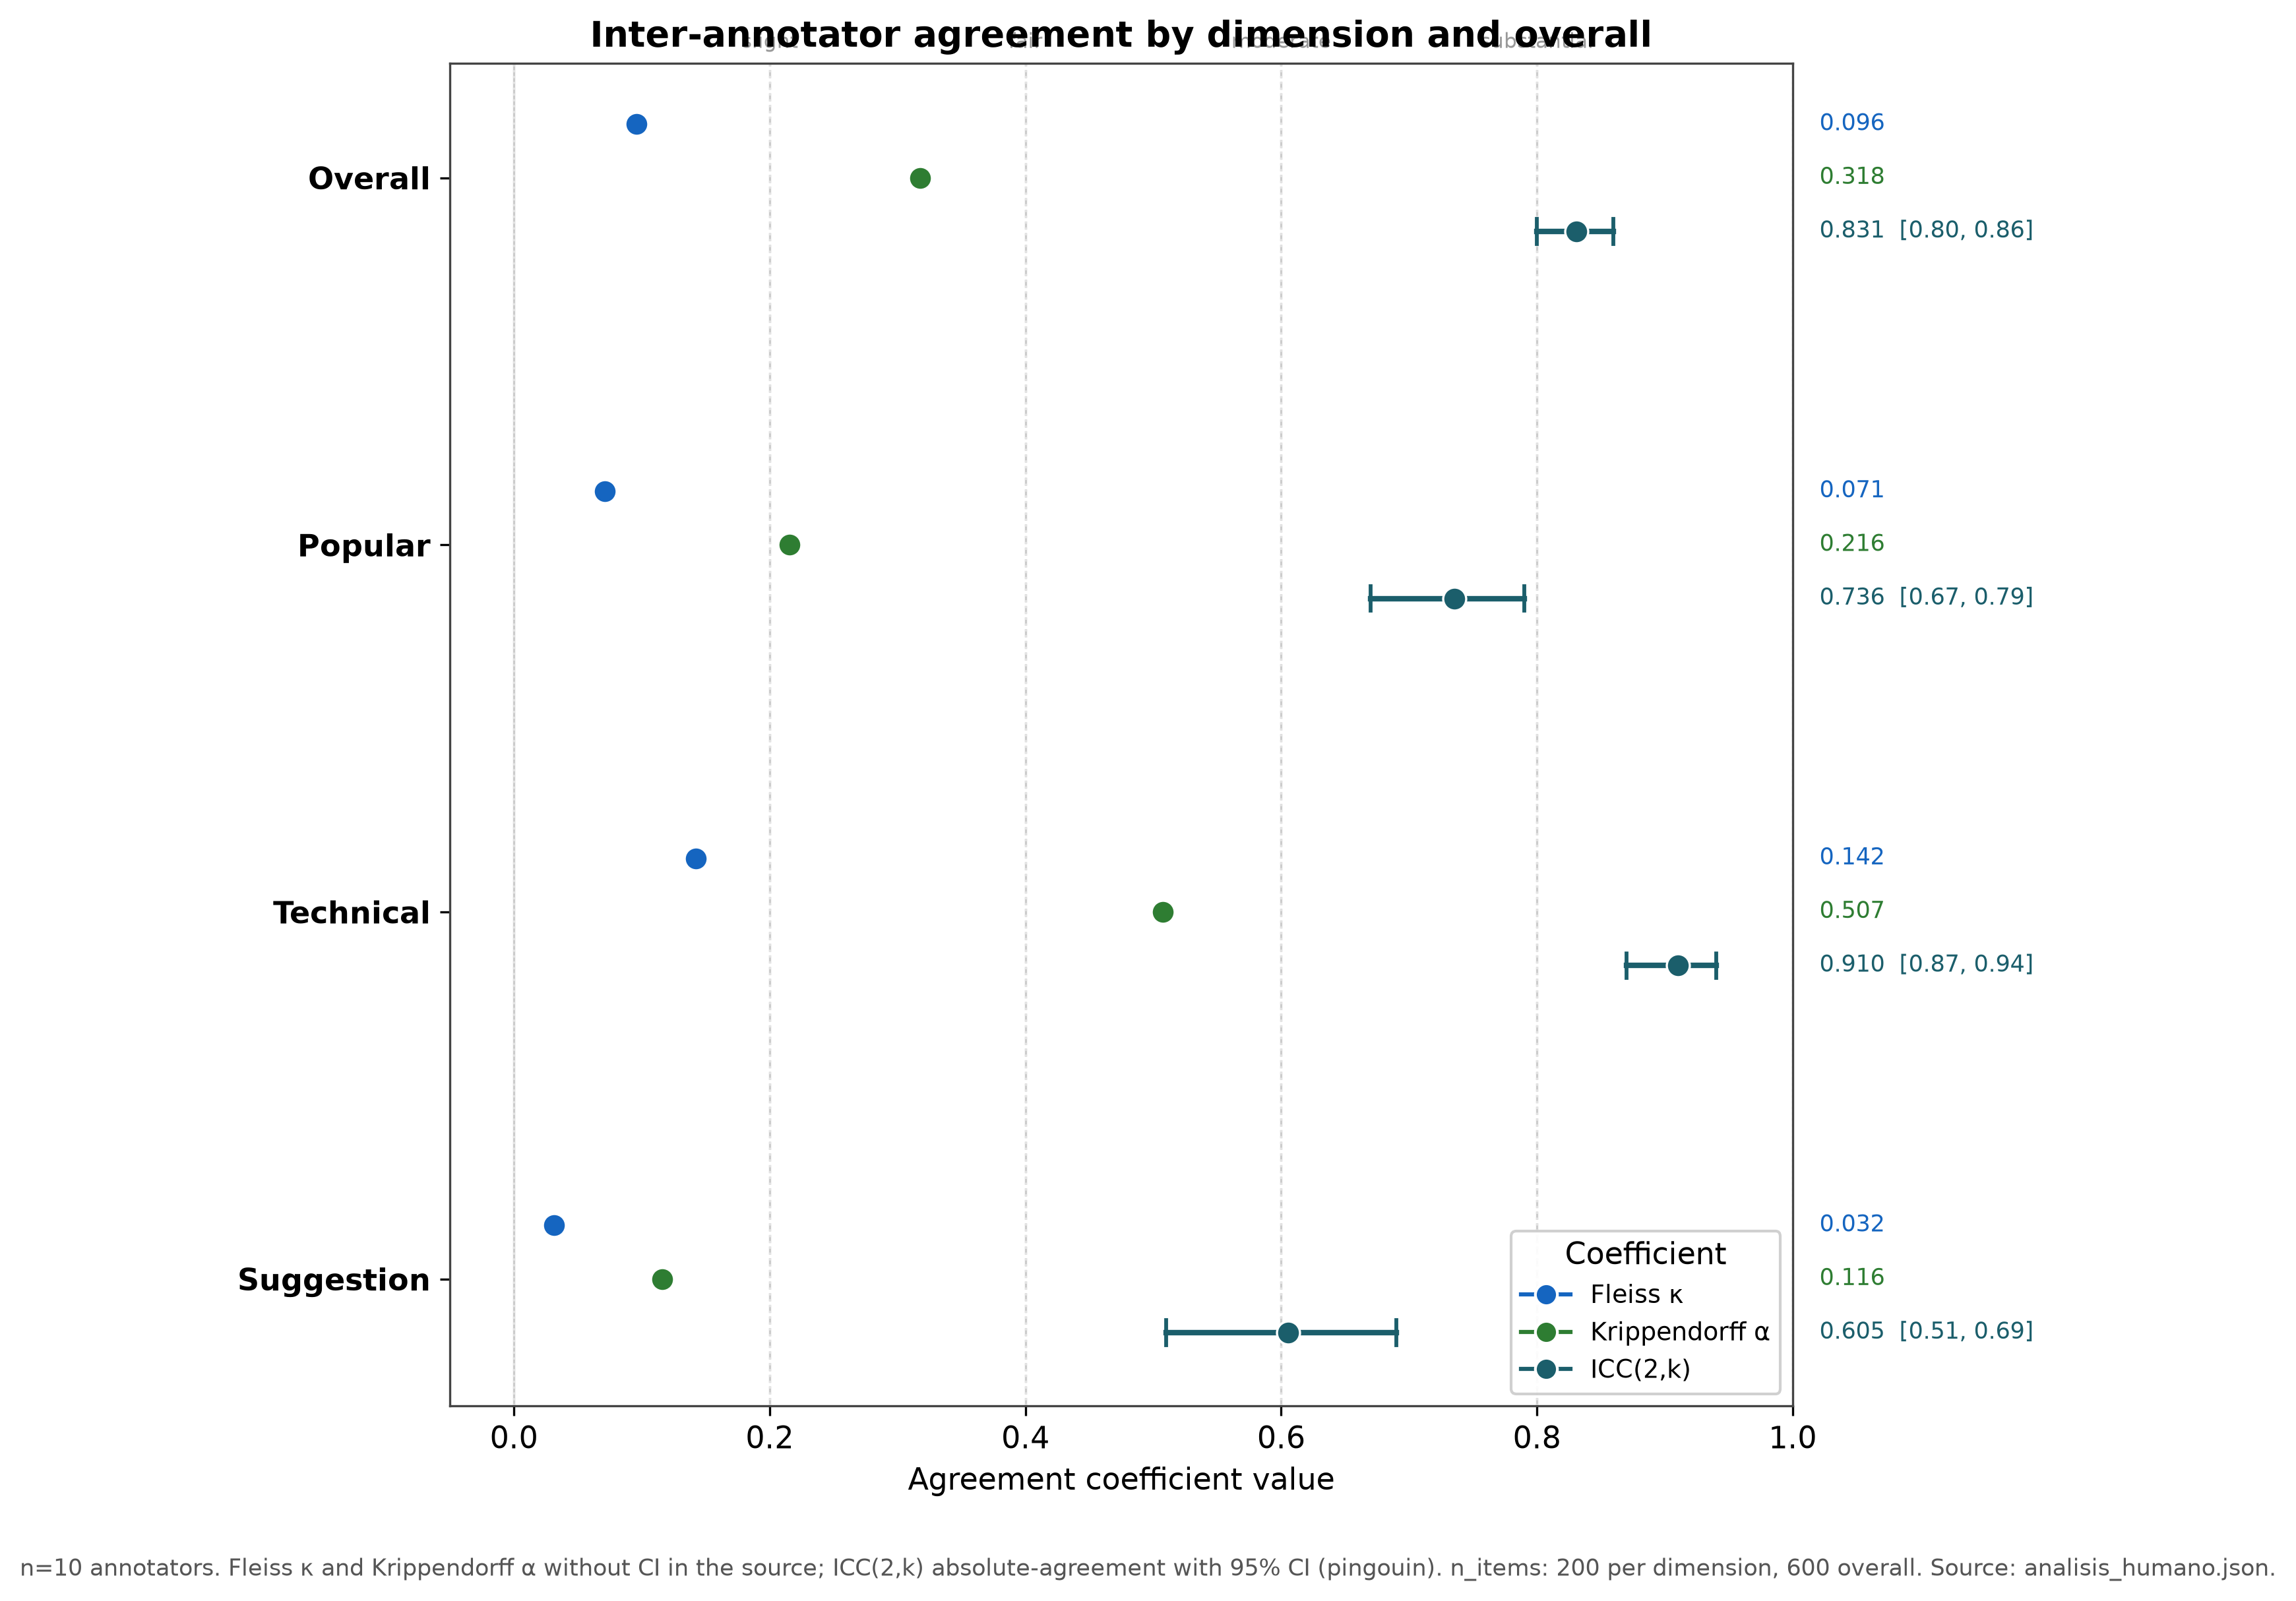
\includegraphics[width=\linewidth]{figs/fig_forest_acuerdo_en.png}
\caption{Inter-annotator agreement among the ten human reviewers by dimension. Fleiss' $\kappa$ and Krippendorff's $\alpha$ (per-rater statistics) are low---especially on the popular and suggestion dimensions---whereas ICC(2,$k$), the reliability of the averaged ten-rater panel, is high (technical 0.910, global 0.831), the central reliability finding of the study.\label{fig:forest}}
\end{figure}

\begin{figure}[H]
\centering
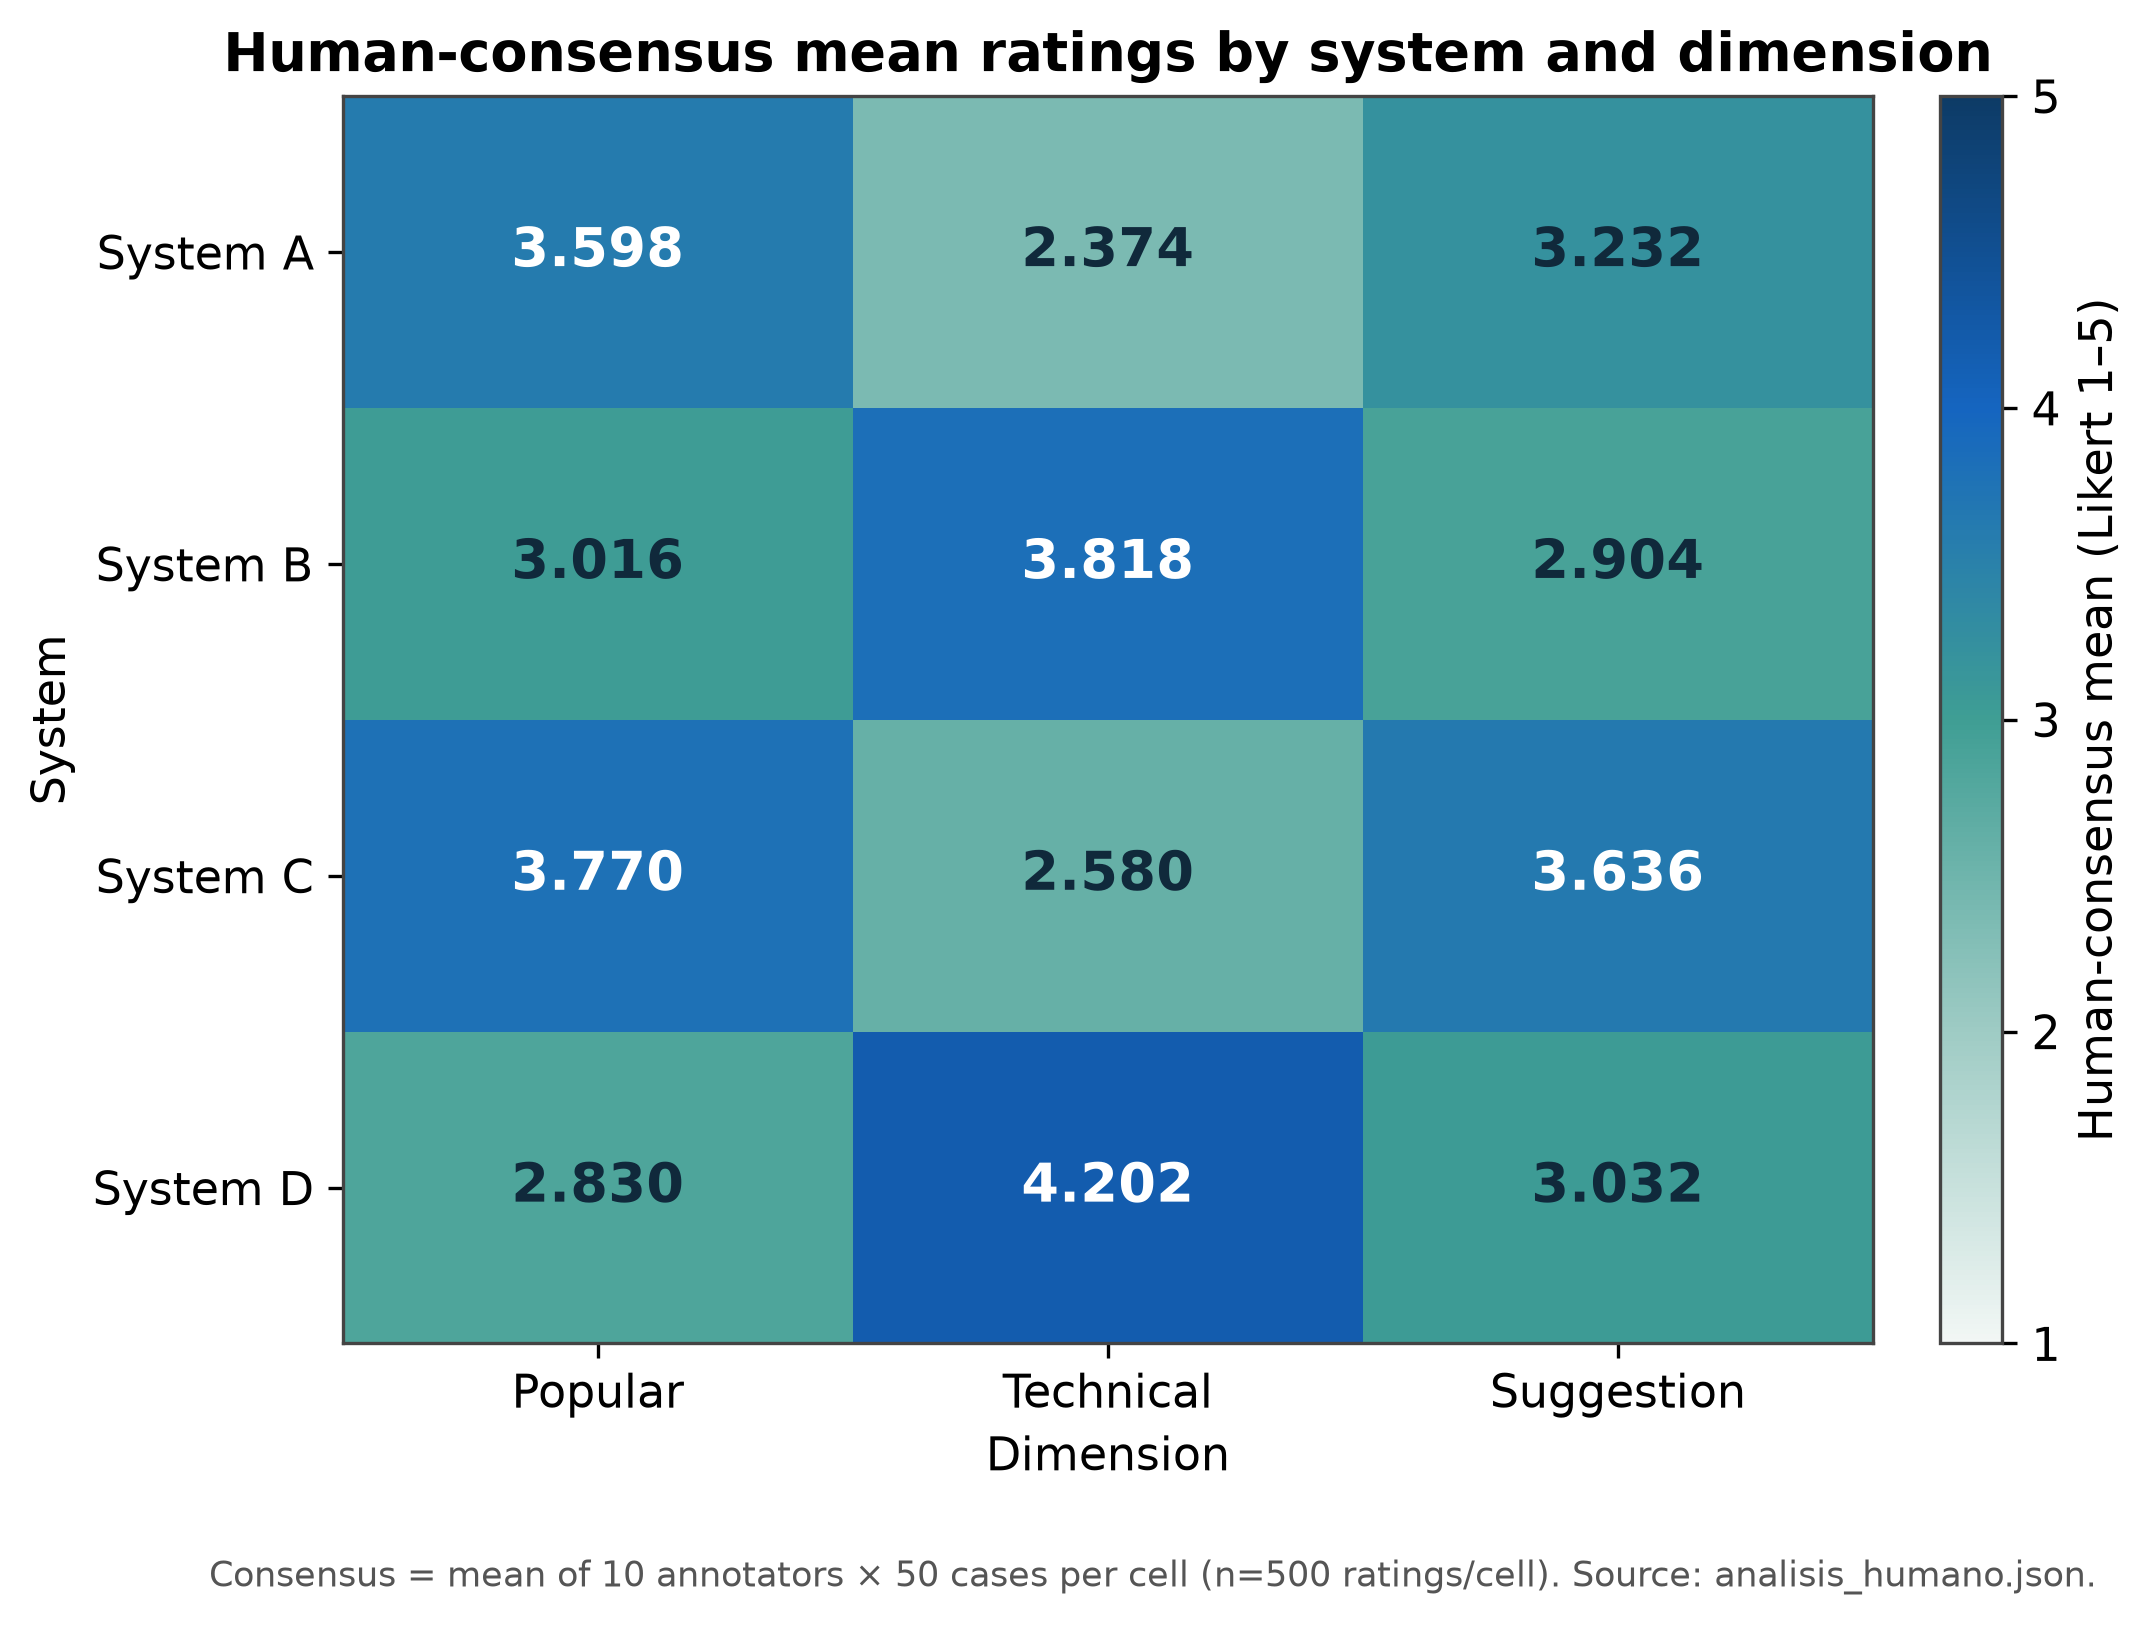
\includegraphics[width=\linewidth]{figs/fig_heatmap_sistema_dimension_en.png}
\caption{Human-consensus mean ratings (1--5) for each system $\times$ dimension. The fine-tuned and hybrid systems (B, D) lead on the technical dimension, while the base and GraphRAG systems (A, C) lead on the popular and suggestion dimensions, the interpretable profile the averaged panel discriminates.\label{fig:heatmap}}
\end{figure}

\emph{The human panel discriminates the systems.} The averaged panel separates the four systems clearly on every dimension, with the Friedman test significant throughout ($\chi^2=122.3$, $137.8$ and $92.6$ for the popular, technical and suggestion dimensions) and all six pairwise system contrasts significant per dimension under Holm-corrected Wilcoxon tests. Across the three dimensions, the human consensus means trace an interpretable profile: on the technical dimension the fine-tuned and hybrid systems lead (D 4.20, B 3.82) over the base and GraphRAG (A 2.37, C 2.58), while on the popular and suggestion dimensions the ordering favours C and A. This is the behaviour expected of a usable instrument: low per-rater agreement, but a reliable and discriminating panel mean. The per-system distribution of human ratings is shown in Figure~\ref{fig:box} and the four-way dimensional profile in Figure~\ref{fig:radar}. RQ4 is answered affirmatively.

\begin{figure}[H]
\centering
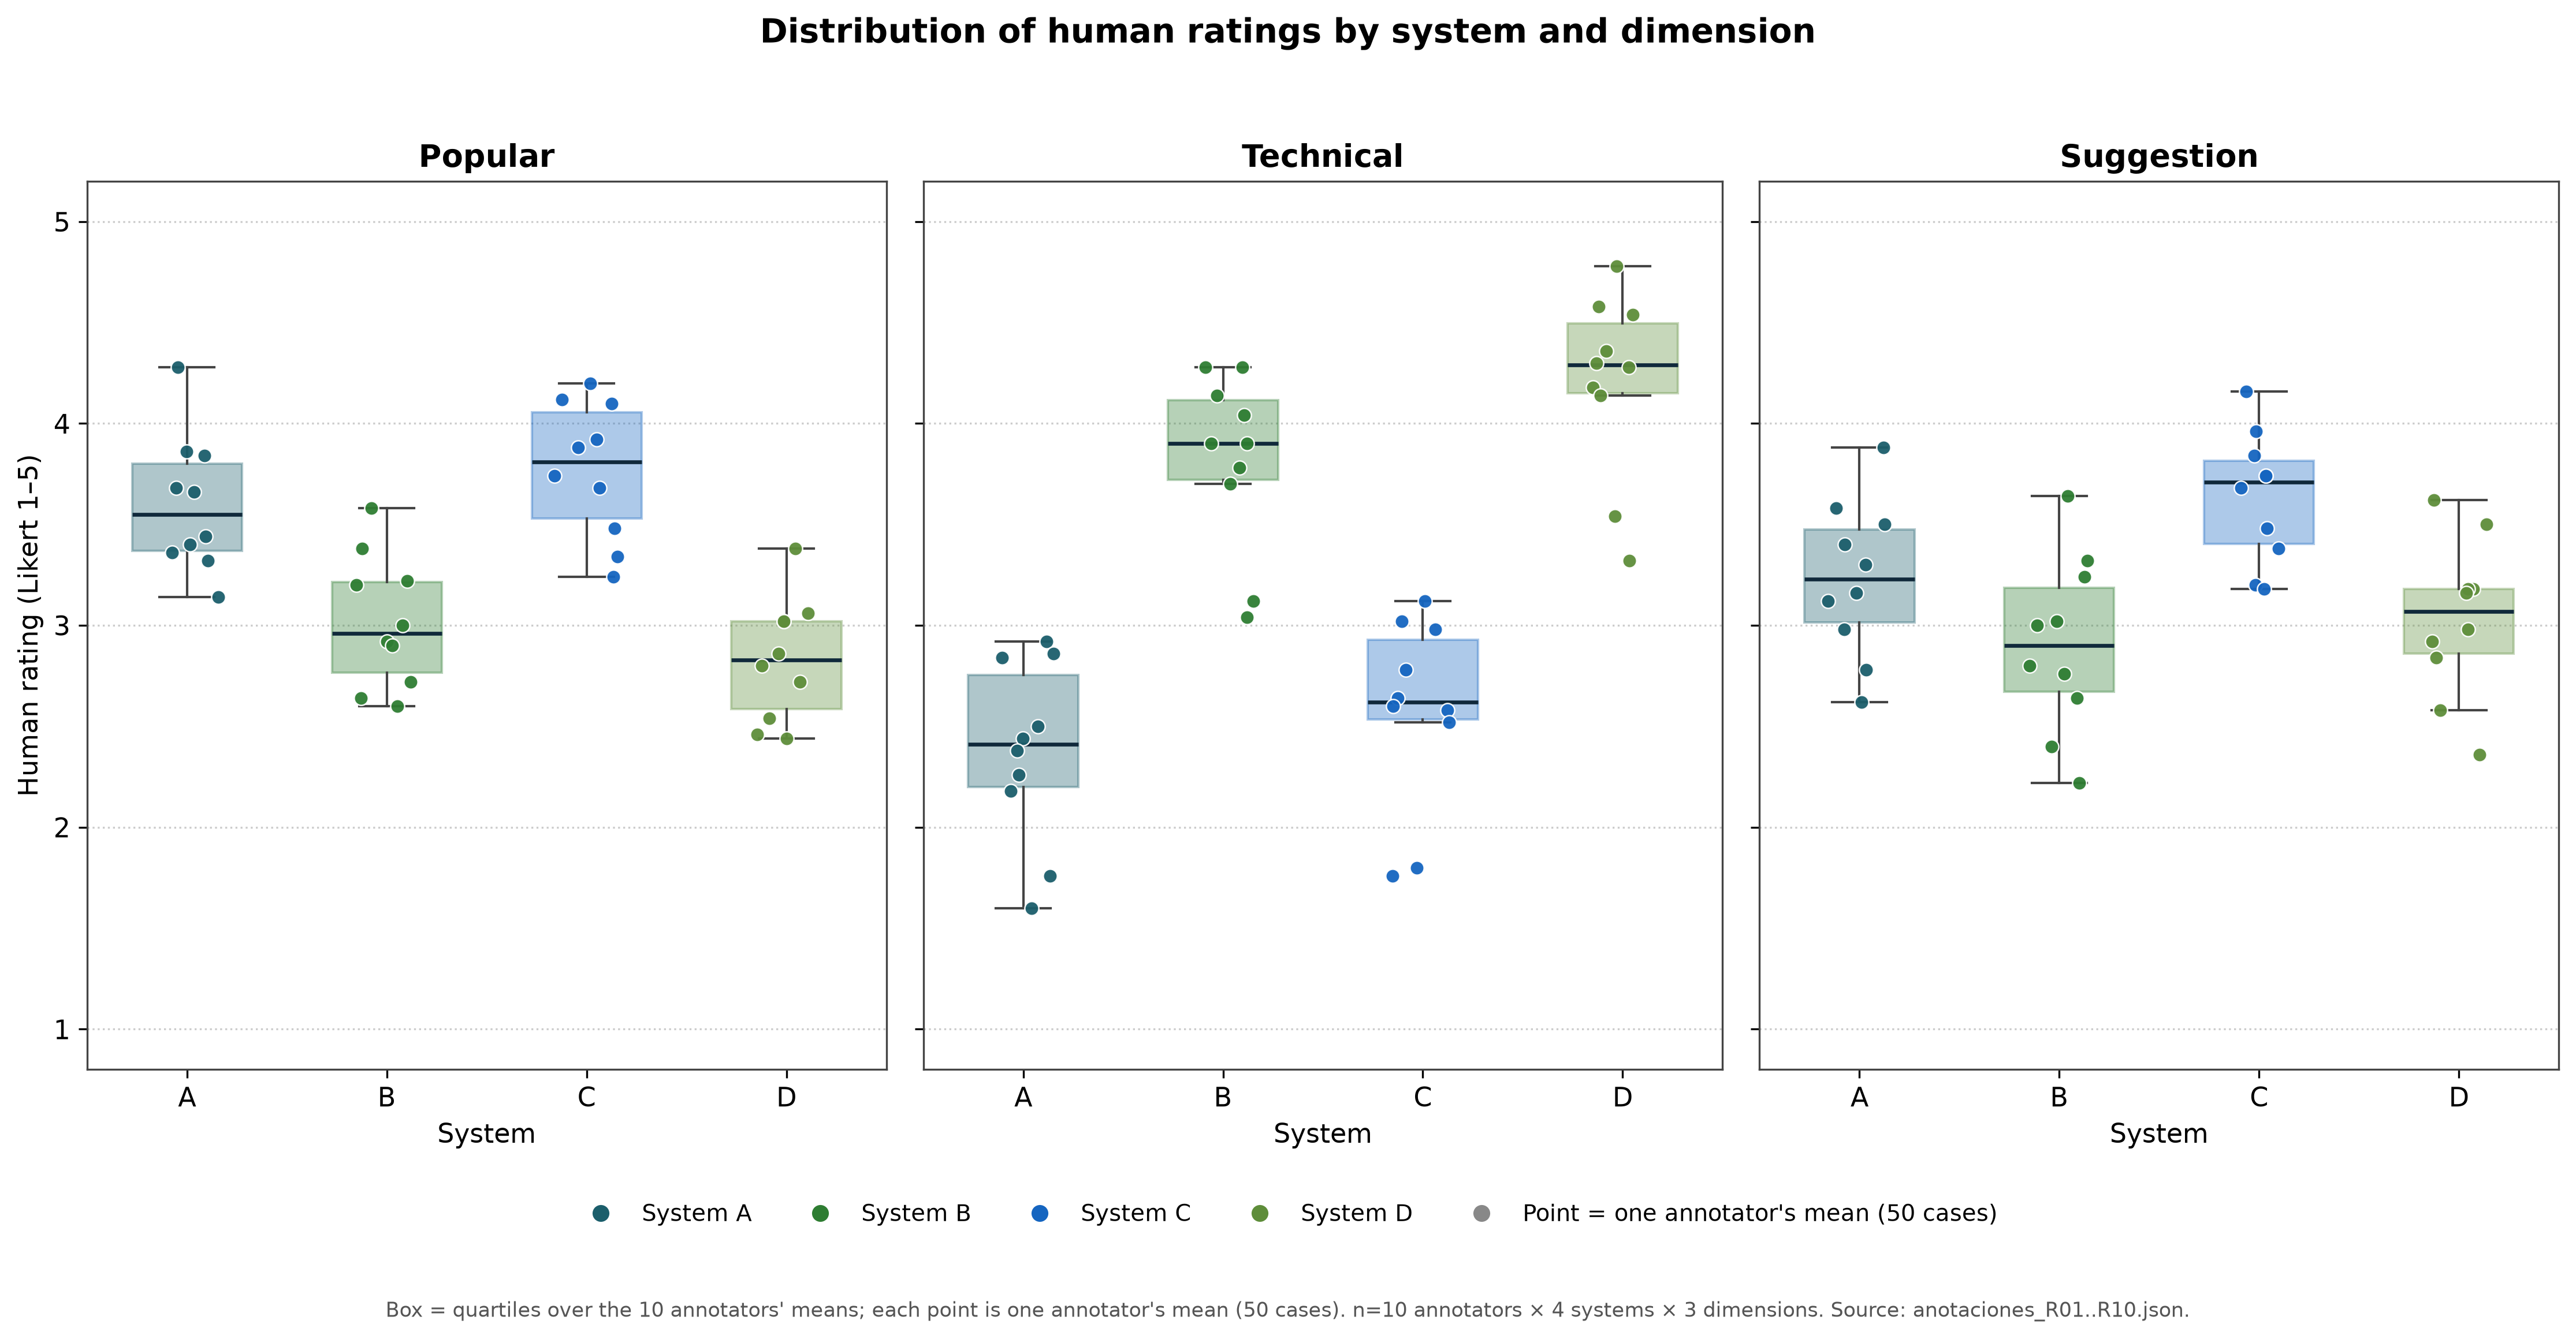
\includegraphics[width=0.95\linewidth]{figs/fig_box_sistemas_en.png}
\caption{Distribution of human consensus ratings across the four systems. The boxplots make the discrimination of the averaged panel concrete: the systems separate clearly despite the modest per-rater agreement.\label{fig:box}}
\end{figure}

\begin{figure}[H]
\centering
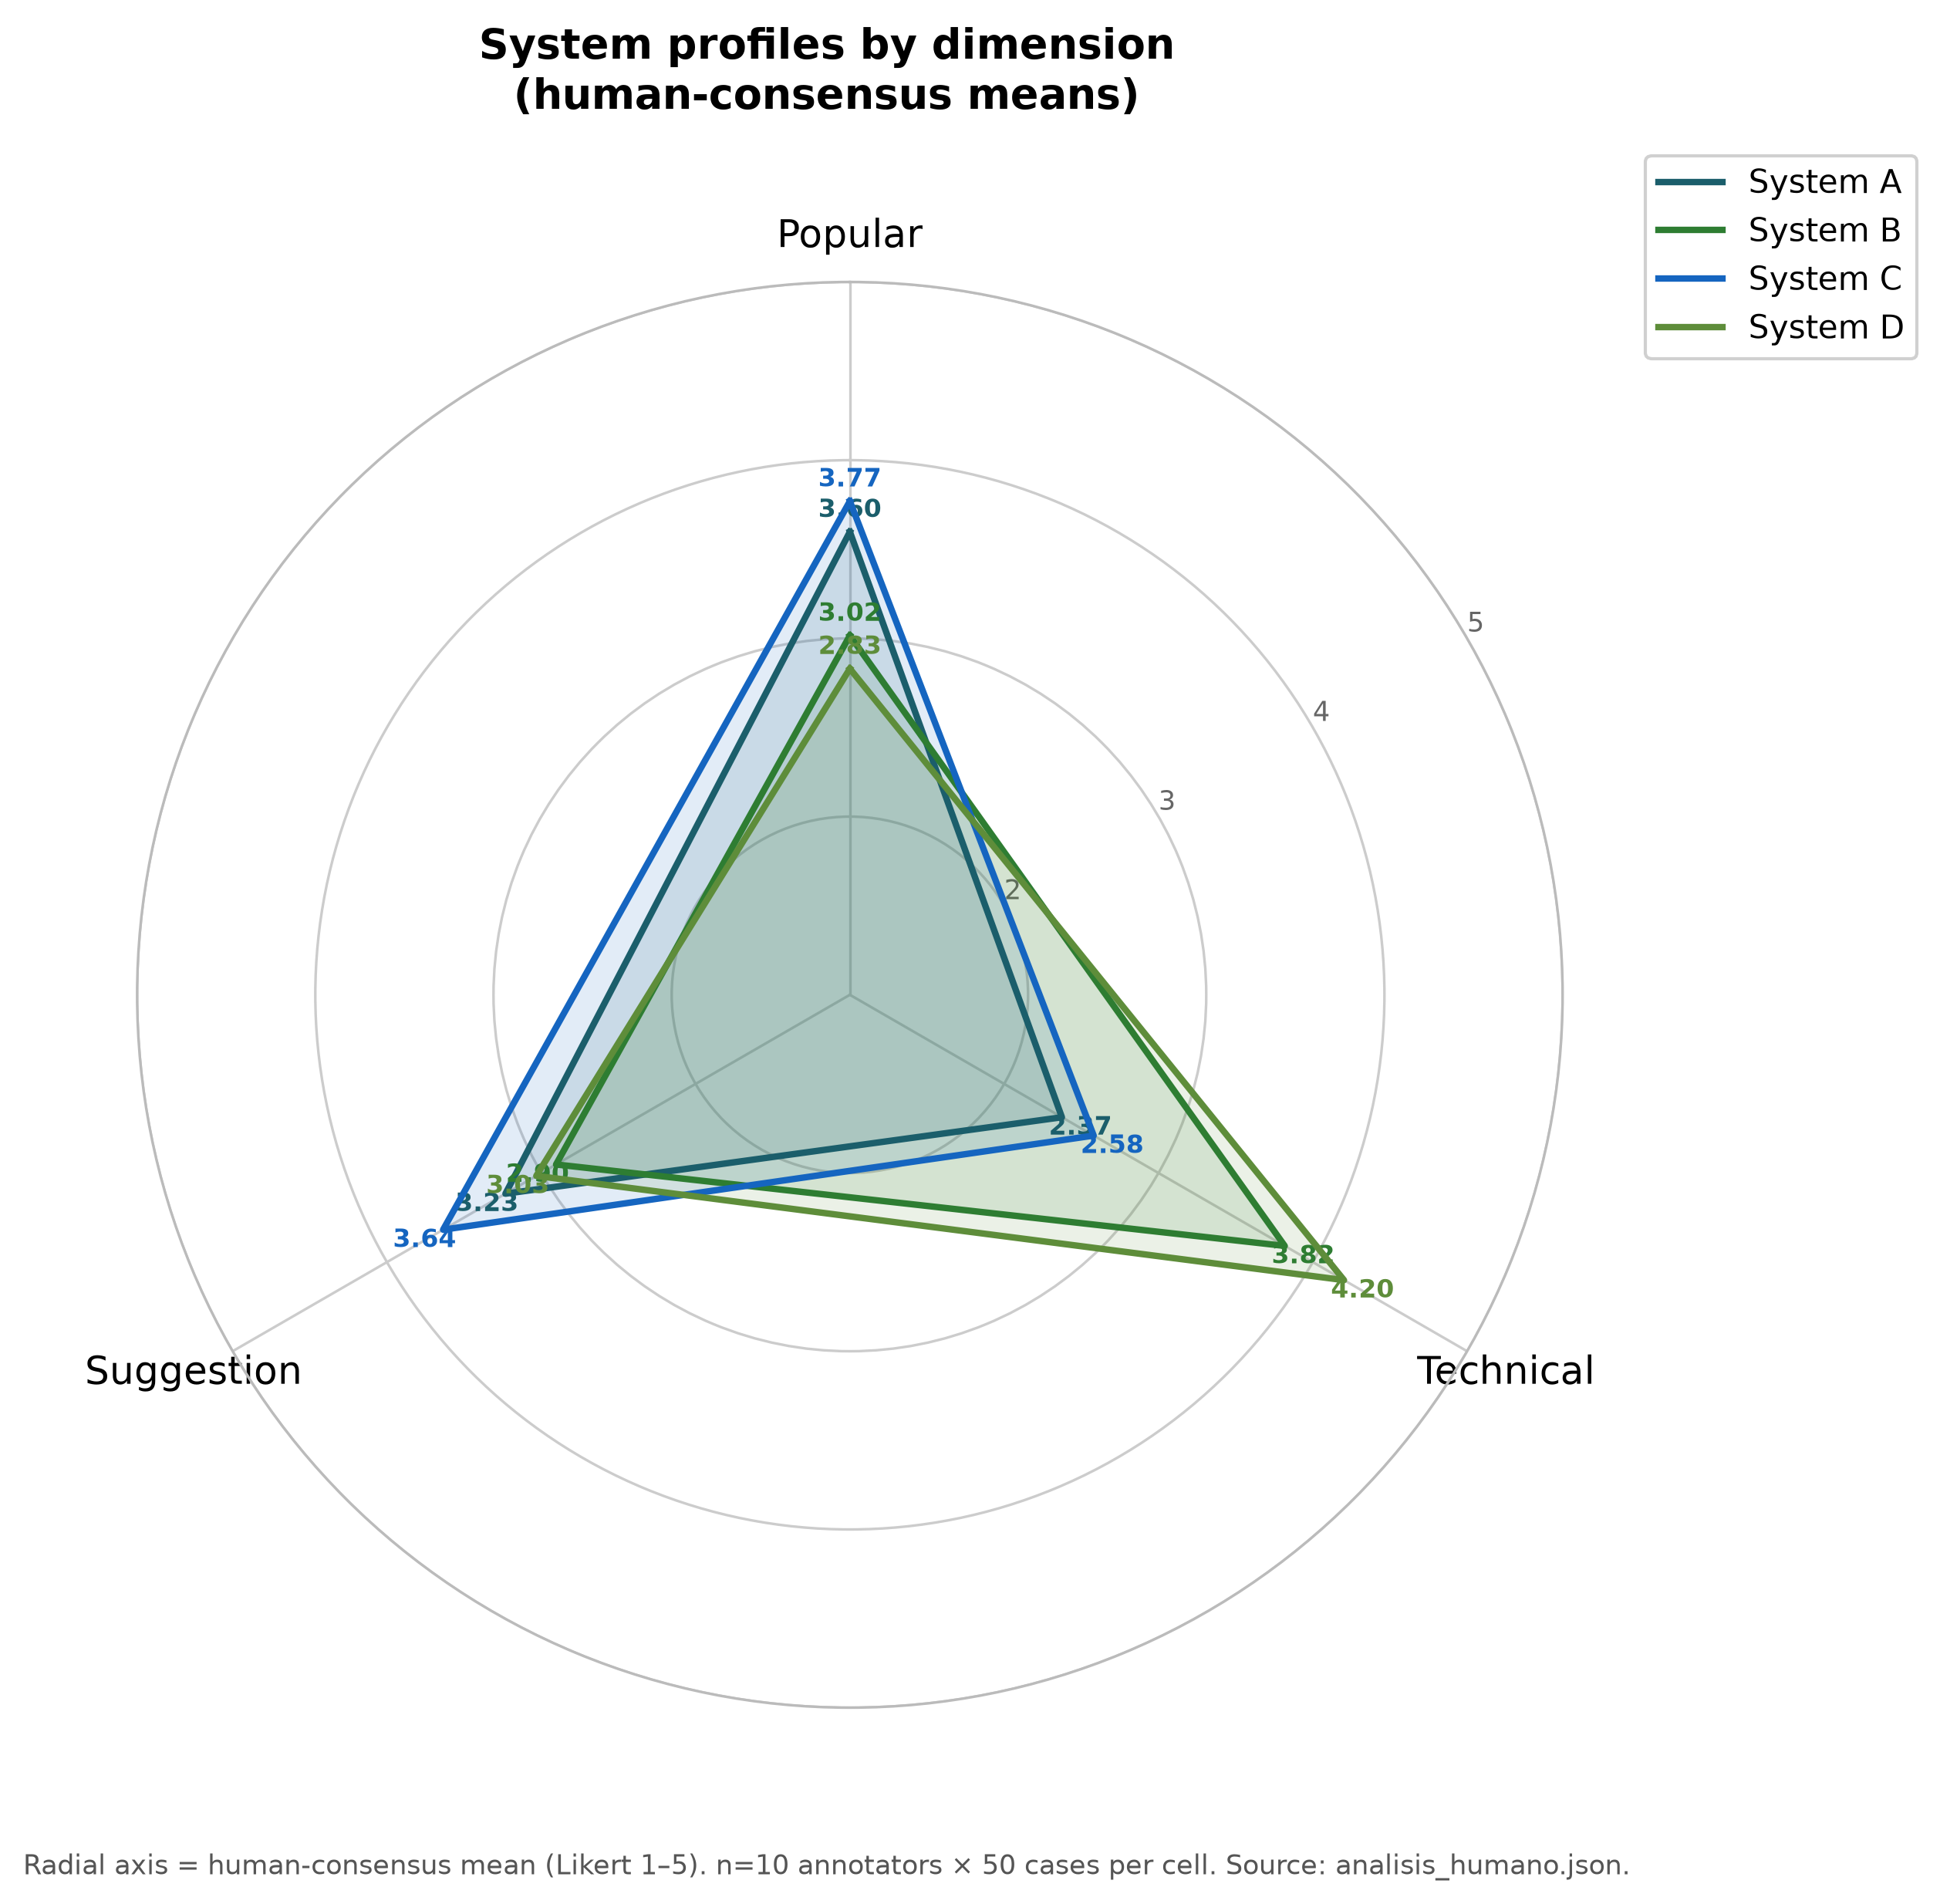
\includegraphics[width=0.72\linewidth]{figs/fig_radar_sistemas_en.png}
\caption{Radar profile of the four systems over the three human-rated qualitative dimensions (popular, technical, suggestion). No single system dominates all dimensions: the fine-tuned and hybrid systems excel on the technical axis while the base and GraphRAG systems lead on the popular and suggestion axes.\label{fig:radar}}
\end{figure}

\emph{Human$\leftrightarrow$judge criterion validity is poor.} Against the human consensus, the LLM judge is not validated as an absolute scoring instrument. The global Pearson correlation is only $0.203$ (Spearman $0.189$). On the popular-explanation dimension it is \emph{negative} ($-0.203$), meaning the judge orders cases inversely to the humans there, while only the technical dimension reaches a moderate $0.363$. Bland--Altman analysis gives a mean bias of $+0.139$ (human minus judge) with limits of agreement of roughly $\pm2.3$ on a 1--5 scale, wide enough to be unusable at the level of an individual cell, as Figure~\ref{fig:bland} shows. RQ3 is therefore answered in the negative for absolute scoring: the judge cannot be assumed to track human educators.

\begin{figure}[H]
\centering
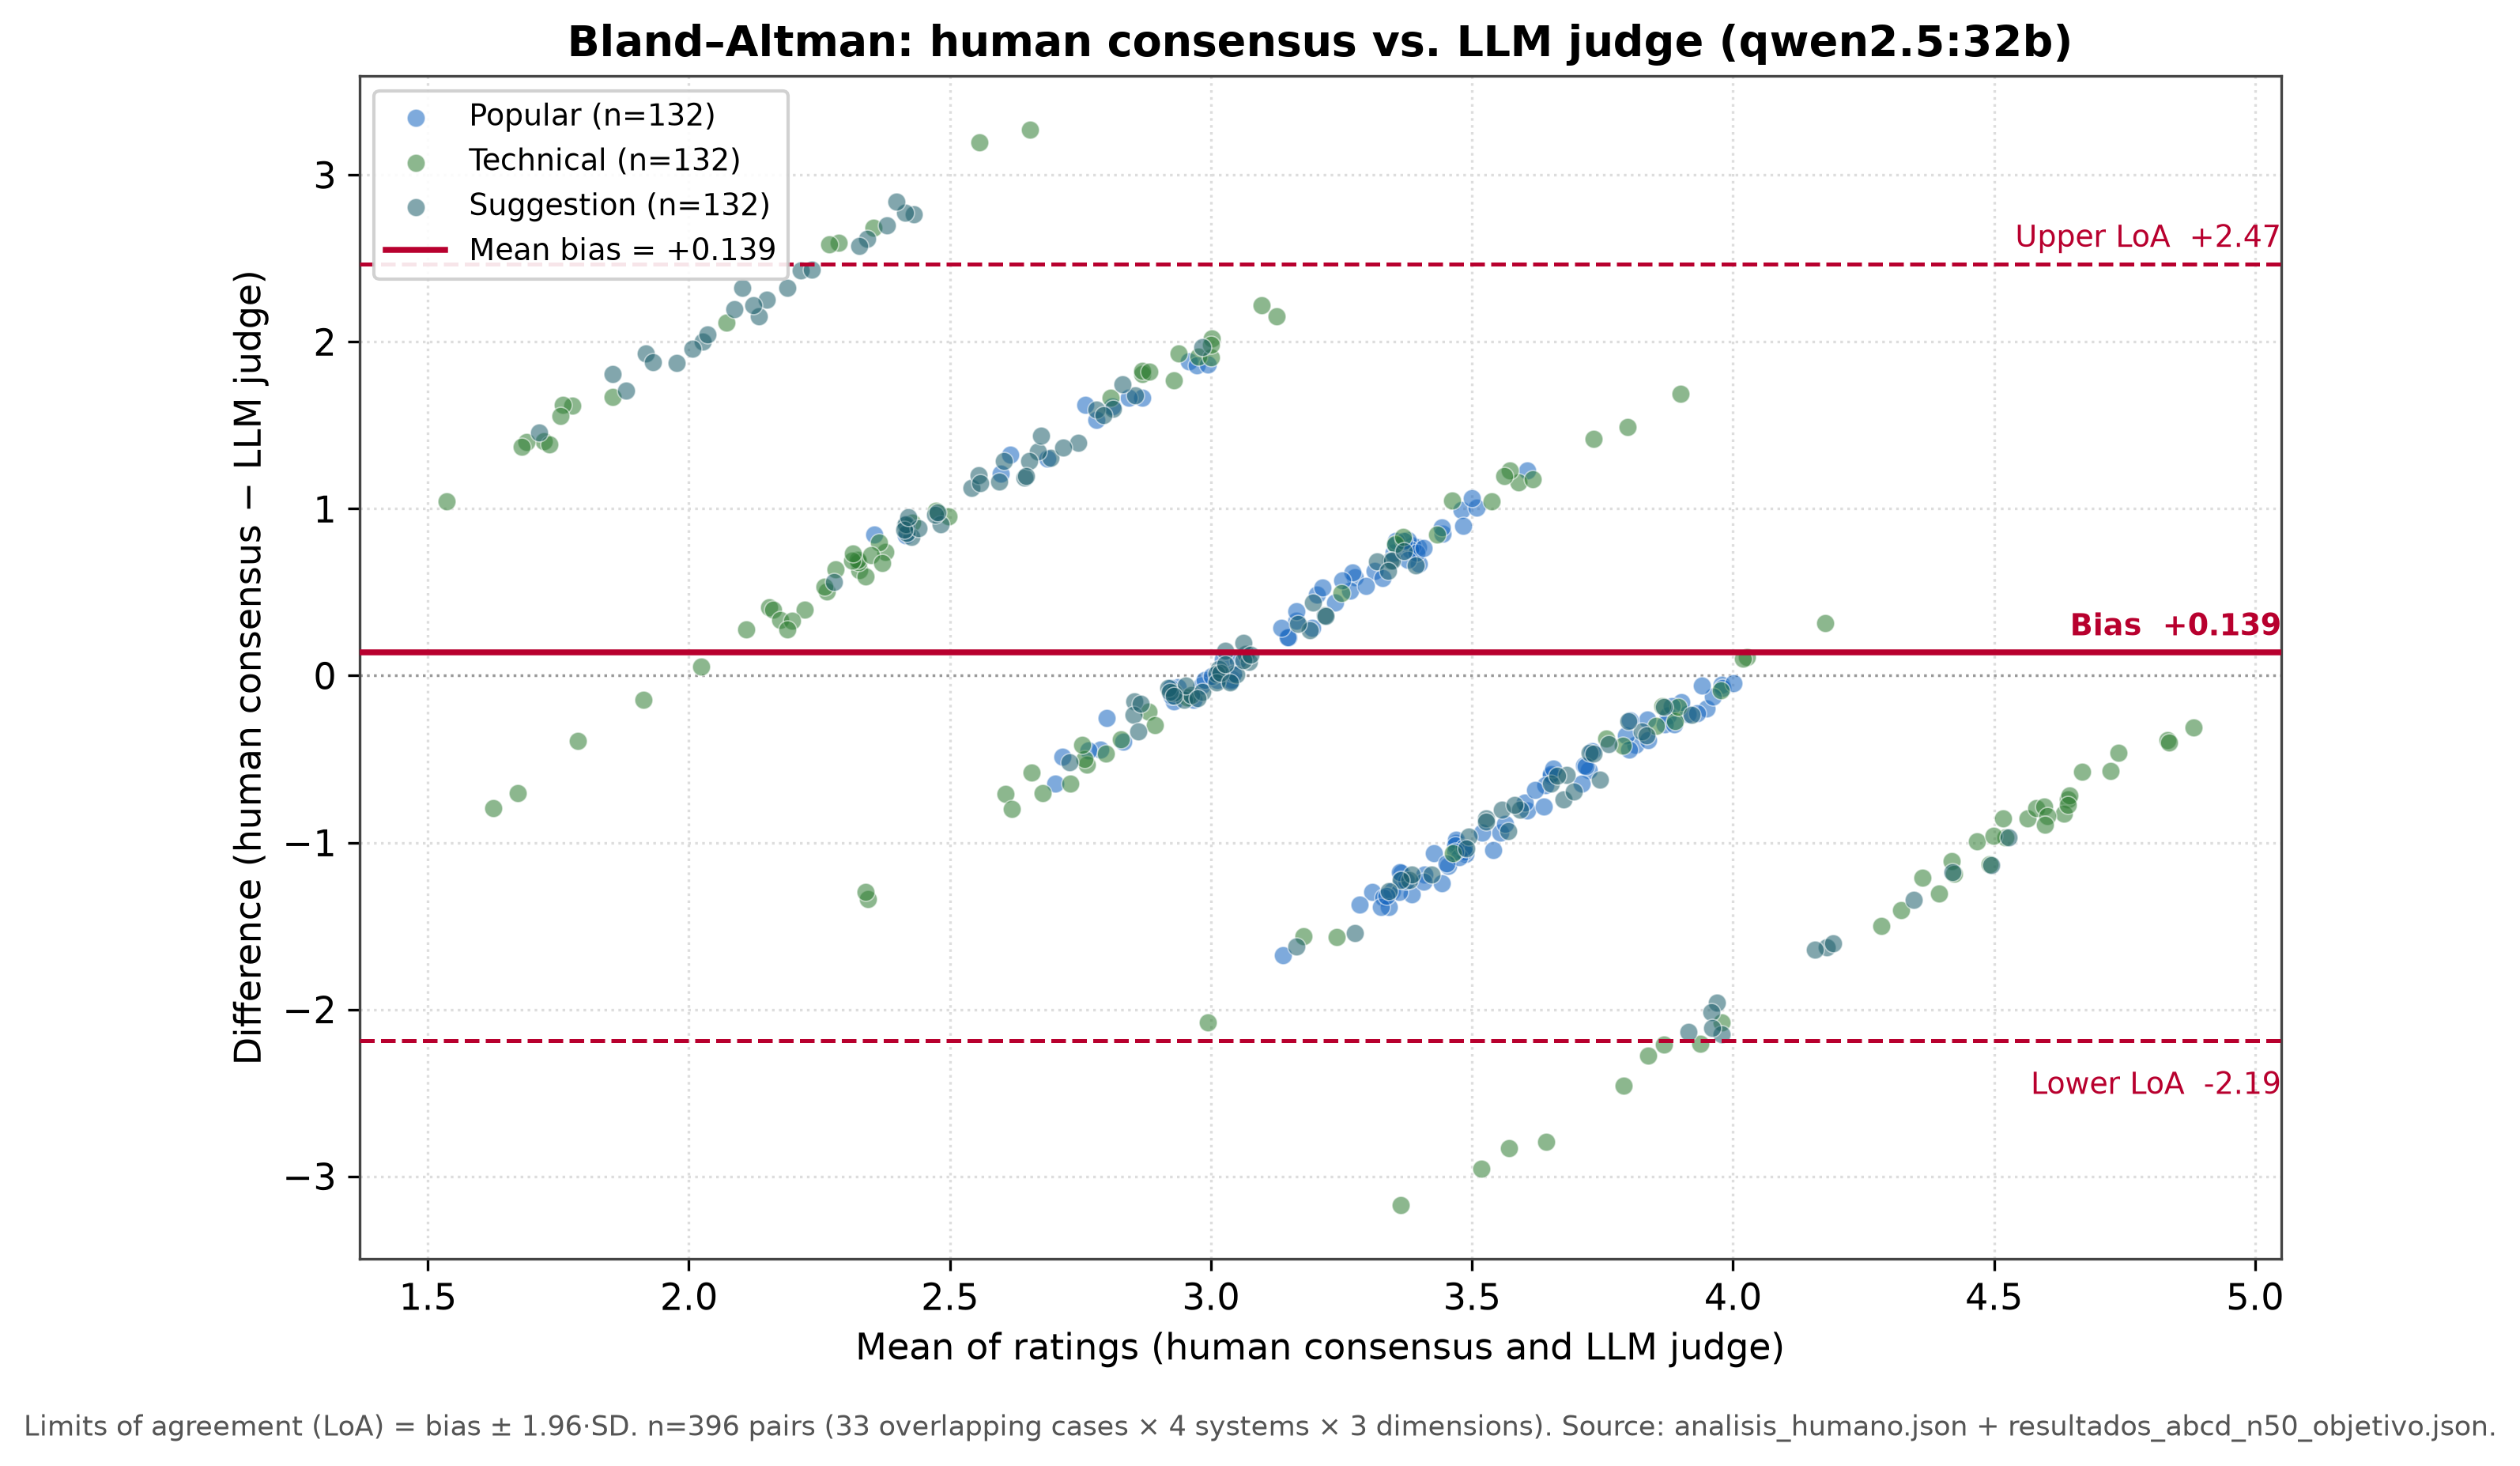
\includegraphics[width=\linewidth]{figs/fig_bland_altman_en.png}
\caption{Bland--Altman agreement between the human consensus and the LLM judge over the 33 overlapping cases. The mean bias is small ($+0.139$, human minus judge), but the limits of agreement (mean $\pm$ 1.96\,SD, $[-2.19,+2.47]$) span almost the full 1--5 range, so the judge and the human panel cannot be treated as interchangeable instruments at the level of an individual rating.\label{fig:bland}}
\end{figure}

\emph{The alternative-annotator substitution test, read alongside the criterion validity.} The formal alternative-annotator (Alt-Test) substitution test of Calderon et al.\cite{calderon2025alttest} was executed with the ten human annotators ($\varepsilon=0.15$). It returns a \emph{global winning rate of 1.0} (the judge wins against all ten annotators, with a mean advantage probability of 0.696) and so concludes ``substitution justified''. The per-dimension winning rates are 1.0 for the popular explanation, 0.6 for the technical explanation and 0.7 for the suggestion (Table~\ref{tab:alttest}). That favourable verdict must be read \emph{together with} the poor criterion validity above, not in isolation, because the two tests measure different things and do not in fact contradict each other. The Alt-Test is a \emph{relative} test: it pits the judge against human annotators who themselves agree very little (Fleiss' $\kappa=0.096$), and when inter-human agreement is that low, ``matching a typical annotator'' is a low bar that an internally consistent judge clears, whereas ``matching the consensus'' (the criterion validity) remains hard (Pearson 0.203). The weighted human$\leftrightarrow$judge $\kappa$ points the same way (global $+0.161$, and \emph{negative} on the popular dimension at $-0.173$, agreeing in sign with the negative Pearson there). The joint reading is therefore that the judge is more consistent than any single isolated human but does not track the order of the consensus and scores systematically high (Bland--Altman $+0.139$). The Alt-Test does \emph{not} rescue the judge as an absolute instrument. Its qualitative scores remain indicative, not definitive, and the verdict is anchored in the objective metrics that are immune to the judge. Reporting the favourable Alt-Test without this nuance would mislead, which is why the two are presented side by side.

\begin{table}[t]
\centering
\caption{Alternative-annotator (Alt-Test) substitution test of the LLM judge against the ten human annotators\cite{calderon2025alttest} ($\varepsilon=0.15$). The global winning rate of 1.0 nominally justifies substitution, but the Alt-Test is \emph{relative} to a panel that agrees very little (Fleiss' $\kappa=0.096$); it must be read together with the weak criterion validity in Table~\ref{tab:reliability}, not as evidence that the judge is a valid absolute instrument.\label{tab:alttest}}
\begin{tabular}{@{}lcccc@{}}
\toprule
Quantity & Global & Popular & Technical & Suggestion \\
\midrule
Winning rate          & \textbf{1.0} & 1.0 & 0.6 & 0.7 \\
Mean advantage prob.\ & 0.696 & 0.781 & 0.680 & 0.626 \\
\bottomrule
\end{tabular}
\end{table}

\begin{table}[t]
\centering
\caption{Reliability and human$\leftrightarrow$judge criterion validity. The averaged human panel is reliable (ICC(2,$k$) 0.831) even though per-rater $\kappa$ is low; the judge's criterion validity against humans is weak and partly negative.\label{tab:reliability}}
\begin{tabular}{@{}lc@{}}
\toprule
Quantity & Value \\
\midrule
Inter-judge Fleiss $\kappa$ (multi-family) & 0.213 \\
Human inter-rater Fleiss $\kappa$ (n=10)   & 0.096 \\
Human Krippendorff $\alpha$ (ordinal)      & 0.318 \\
Human ICC(2,k) absolute agreement          & 0.831 \\
Human$\leftrightarrow$judge Pearson $r$    & 0.203 \\
\quad popular-explanation dimension        & $-0.203$ \\
\quad technical-explanation dimension      & $+0.363$ \\
Bland--Altman bias (human $-$ judge)       & $+0.139$ \\
Overlapping cases (human $\cap$ judge)     & 33/50 \\
\bottomrule
\end{tabular}
\end{table}

The per-dimension breakdown of the three human inter-annotator coefficients is given in Table~\ref{tab:agreement}. It exposes the same pattern more finely: the technical dimension is by far the most reliable (ICC 0.910, $\alpha$ 0.507), the suggestion dimension the least (ICC 0.605, $\alpha$ 0.116), and the gap between the low per-rater Fleiss' $\kappa$ and the high panel ICC holds on every dimension. The ordering of reliability across dimensions matches the ordering of human$\leftrightarrow$judge correlation, supporting the reading that judge validity is bounded above by the inherent rateability of each dimension.

\begin{table}[t]
\centering
\caption{Human inter-annotator agreement by dimension (ten reviewers, 6000 dimension-level ratings). Per-rater coefficients (Fleiss' $\kappa$, Krippendorff's $\alpha$) are low, but the averaged-panel reliability ICC(2,$k$) is high---most so on the technical dimension, least on the suggestion dimension.\label{tab:agreement}}
\begin{tabular}{@{}lcccc@{}}
\toprule
Coefficient & Global & Popular & Technical & Suggestion \\
\midrule
Fleiss' $\kappa$              & 0.096 & 0.071 & 0.143 & 0.032 \\
Krippendorff's $\alpha$       & 0.318 & 0.216 & 0.507 & 0.116 \\
ICC(2,$k$) abs.\ agreement    & \textbf{0.831} & 0.736 & \textbf{0.910} & 0.605 \\
\bottomrule
\end{tabular}
\end{table}

%% =========================================================================
\section{Discussion}
%% =========================================================================

\subsection{Synthetic versus real, and why augmentation helps in distribution but not out of it}
The two benchmarks tell a coherent story once the diversity audit is taken into account. In distribution, augmentation works. Fine-tuning improves error-type classification, graph grounding lifts concept identification and traceability, and the hybrid combines both to lead the synthetic benchmark, with all augmented systems significantly beating the base LLM. Out of distribution, the ranking inverts and the inversion is statistically significant. What reconciles the two is the measured intra-skeleton homogeneity of the synthetic training data (cosine 0.962 within skeletons against 0.604 globally): the fine-tuned generator learned the \emph{format} of a small set of templates rather than a generalisable feedback competence, so its advantage evaporates on the heterogeneous real corpus. This is a textbook over-fitting diagnosis, and testing out of distribution is what converts a suspicion into a measured, significant result. The caveat cuts both ways: because the fix-relevance metric rewards literal token overlap with the educator's diff, and the fine-tuned systems were trained to give conceptual explanations instead of echoing the student's code, part of the gap is a difference in feedback style more than in correctness. The objective signal nonetheless stands, and it constrains the central claim to ``augmentation helps in distribution,'' not ``the hybrid is best in general.''

\subsection{The validity of automated educational evaluation}
The reliability findings are, taken together, the study's main methodological result, and they are asymmetric. On one side, the LLM judge is not a valid absolute instrument: its agreement with the human consensus is weak (Pearson 0.203), is negative on the popular-explanation dimension, and has Bland--Altman limits of agreement too wide to trust any single cell; moreover the judge's own scores depend heavily on which model family is asked, with multi-family Fleiss' $\kappa=0.213$ and reproduced pairwise agreement of 0.118. This converges with, and supplies domain-specific evidence for, the critical literature that questions the validity and reliability of LLM judges as measurement instruments.\cite{chehbouni2025neither,li2025scoringbias,hackl2023gpt4,yamauchi2025judge} One result apparently dissents. The alternative-annotator substitution test of Calderon et al.,\cite{calderon2025alttest} which returns a global winning rate of 1.0 and a verdict of ``substitution justified'' (Table~\ref{tab:alttest}), does not in fact overturn this conclusion, and reporting it as though it did, or omitting it, would mislead. The Alt-Test is \emph{relative}: it asks only whether the judge is at least as aligned with the rest of the panel as a typical individual annotator is, and against a panel whose own inter-rater agreement is as low as Fleiss' $\kappa=0.096$ that is a low bar. An internally consistent judge clears it because each isolated human is noisy, while tracking the \emph{consensus} (the criterion validity, Pearson 0.203) stays hard. The weighted human$\leftrightarrow$judge $\kappa$ confirms the reading, being only $+0.161$ globally and \emph{negative} ($-0.173$) on the popular dimension, in sign agreement with the negative Pearson there. The favourable Alt-Test therefore certifies that the judge beats an isolated human, not that it is a valid absolute instrument. It must be read beside, never instead of, the weak criterion validity, and the qualitative judge scores remain only indicative. On the other side, the averaged human panel \emph{is} reliable (ICC(2,$k$) 0.831) and discriminates the systems with significance, even though per-rater Fleiss' $\kappa$ is only 0.096. The apparent paradox of low per-rater $\kappa$ alongside high panel ICC follows directly from how the two statistics are defined: a fine-grained 1--5 scale depresses exact categorical agreement between individuals, while averaging ten raters cancels their idiosyncratic noise and leaves a stable signal.\cite{shrout1979icc,mcgraw1996icc,fleiss1971kappa} We draw a sharp practical lesson: a single rater, whether an LLM judge or one human, is an unsafe basis for a quality verdict on programming feedback, whereas an averaged human panel is a sound one. The one dimension where humans agree most (technical, ICC 0.910) is the one where the judge correlates best with them (0.363), suggesting that judge validity is bounded above by the inherent rateability of the dimension.

\subsection{Implications and comparison with prior work}
For practitioners, the immediate implication is that verdicts about LLM-generated educational feedback should be anchored in objective, ground-truth-anchored metrics and in grounding/faithfulness measures that are immune to the judge, and that qualitative LLM-judge scores should be read as weak, judge-dependent evidence rather than as ground truth. Our recommendation is consistent with, but goes beyond, prior cautions: where much of the LLM-as-a-judge literature establishes judge--judge inconsistency or general bias,\cite{li2024judges,verga2024poll,zheng2023judging} we measure judge--human criterion validity for a generative task with a real ten-person panel and find it wanting. Relative to the educational-feedback literature, which typically reports that augmented or fine-tuned systems improve feedback quality,\cite{sahu2025autograder,scholz2025partnering,yu2025codereview,phung2023feedback} our two-distribution design qualifies such claims by showing that an in-distribution improvement certified even by objective metrics need not survive contact with real student code. And relative to the knowledge-graph-in-education and GraphRAG literature,\cite{qu2024survey,cheng2025graphrag,peng2024graphrag,pan2024unifying} the contribution is a validated, reasoning-closed artefact whose grounding is empirically quantified, with the retriever's modest context precision (0.375) identified as the next target. More broadly, the panel mean, not any single automated rater, should ground the verdict, a methodological point that transfers beyond programming feedback to any setting where LLM judges are used to evaluate generated educational text.

\subsection{A separate retrieval ablation: passage RAG versus semantic SPARQL RAG (Linaje~B)}
Alongside the canonical A/B/C/D study above, a self-contained reconstruction experiment (referred to here as Linaje~B and kept strictly apart from the canonical figures, so that no number from one experiment is presented as belonging to the other) isolates the effect of \emph{what} is retrieved rather than \emph{whether} fine-tuning helps. Three ORPO-trained variants that all share a single QLoRA adapter (so any difference between them is attributable to retrieval, not to fine-tuning) were judged by \texttt{qwen2.5:32b} on a small held-out set of ten cases, against a no-retrieval base. Two passage-level retrieval variants, ORPO-v2 (retrieving Web-Semantics graph passages) and ORPO-v3 (retrieving Python textbook passages), do \emph{not} improve over the no-retrieval base (global means 3.467 and 3.567 against the base's 3.733): injecting many tangential passages dilutes the context and degrades the answer. A third variant, ORPO-v4, instead retrieves by SPARQL a single surgical pedagogical rule from a small Python misconception ontology, and \emph{does} surpass the base (global mean \textbf{4.233} versus 3.733), with the gain concentrated in the technical (4.8 vs.\ 4.2) and suggestion (3.8 vs.\ 2.8) dimensions and a formatting-fidelity rise (0.94 vs.\ 0.88); on a per-case basis v4 wins, ties or loses against the base 6/2/2. The result carries explicit caveats. The entire improvement is one of \emph{retrieval, not of fine-tuning}, since v4 reuses v3's adapter unchanged. Two genuine regressions of v4 against the base remain (cases \texttt{sub\_00803}, $4.333\rightarrow4.0$, and \texttt{sub\_01444}, $4.333\rightarrow3.667$). Only 3 of the 10 cases activated a specific misconception rule; the sample is small ($n=10$) and the judge is non-deterministic; and the ontology is itself an AI-designed artefact anchored to the dataset's own taxonomy. One narrow but reproducible lesson emerges: semantic, schema-guided retrieval of a minimal relevant unit can help where bulk passage retrieval hurts, complementing, in a different experimental setting, the canonical study's finding that grounding must be measured rather than assumed.

%% =========================================================================
\section{Limitations}
%% =========================================================================
We note several limitations. The synthetic dataset derives from a small set of structural skeletons whose intra-skeleton cosine similarity (0.962) we measured directly, and the consequent in-distribution gains do not transfer to real code, as the significant ranking inversion shows. Sample sizes are modest ($n=50$ synthetic, $n=60$ real), which limits statistical power for system-versus-system contrasts. Most tellingly, the hybrid D's numerical advantage over the fine-tuned B is not significant at $n=50$. The fix-relevance metric on real code rewards literal token overlap and therefore partly penalises the conceptual feedback style that the fine-tuned systems were trained to produce. It should be read as a lower bound on their usefulness, not a verdict on their correctness. The qualitative judge scores carry low reliability (multi-family Fleiss 0.213) and a within-family overlap between the judge and systems B/D, which is why they do not anchor any conclusion. Most important for the criterion-validity claim, the human and judge case sets overlap in only \textbf{33 of 50} cases, so the human$\leftrightarrow$judge analysis is computed over those 33 cases ($\times4$ systems $\times3$ dimensions $=$ 396 cells); closing the overlap to 50/50 is the single remaining step toward full criterion validity, and remains pending. Finally, the evaluation is confined to introductory Python feedback in Spanish from local 7--8B-class models. The alternative-annotator substitution test for the judge\cite{calderon2025alttest} has been executed on the ten available annotators and returns a favourable global winning rate of 1.0, but, as Section~7 explains, this is a \emph{relative} verdict against a low-agreement panel (Fleiss 0.096) and does not validate the judge as an absolute instrument, so it is reported only beside the weak criterion validity and not as a substitution warrant; generalisation to other languages, domains and model scales remains future work.

%% =========================================================================
\section{Conclusion}
%% =========================================================================
We presented a SHACL-validated, OWL~2~RL-closed Educational Knowledge Graph for introductory Python (157 concepts; 1772$\rightarrow$4786 triples; 30 verified \texttt{skos:exactMatch} links; zero SHACL violations) and a GraphRAG feedback pipeline built around it, and we evaluated four systems (a base LLM, a QLoRA-fine-tuned model, GraphRAG and their hybrid) with three independent kinds of evidence: judge-immune objective metrics, an LLM judge probed across model families, and a blind ten-person human panel producing 6000 dimension-level ratings. In distribution the augmentations significantly beat the base LLM and the hybrid leads, but on real student code the objective ranking inverts significantly (Friedman $p=8.1\times10^{-15}$), a measured over-fitting result. Our conclusion is methodological: the LLM judge is \emph{not} validated as an absolute scoring instrument (its agreement with humans is weak and partly negative, and its scores are judge-dependent), whereas the \emph{averaged} human panel is reliable (ICC(2,$k$) 0.831) and discriminates the systems. Verdicts on such systems should therefore rest on objective, ground-truth-anchored metrics and on grounding, with the human panel mean, not any single rater, as the criterion. Future work will close the human/judge overlap to 50/50 to complete the criterion-validity and substitution analyses, and diversify the training data and improve the retriever to address the measured over-fitting and the modest context precision.

%% =========================================================================
\section{Future Work}
%% =========================================================================
Five prioritised directions follow directly from the results, each tied to a measured shortfall. \emph{First}, and most immediately, the human$\leftrightarrow$judge case overlap will be closed from the current 33 of 50 cases to the full 50, so that the criterion-validity correlations and the Bland--Altman analysis are computed over the complete held-out set; this would also let the alternative-annotator substitution test (winning-rate threshold, $\varepsilon=0.15$, $t$-test/Wilcoxon), already executed on the present panel with a favourable but \emph{relative} global winning rate of 1.0, be recomputed over the full overlap, since its favourable verdict against a low-agreement panel does not yet validate the judge as an absolute instrument.\cite{calderon2025alttest} \emph{Second}, the measured over-fitting motivates diversifying the training targets instead of only the code: the intra-skeleton cosine of 0.962 shows that the synthetic ``unique'' targets differ chiefly in variable names, so varied rewording or distillation of feedback from a stronger teacher model is the targeted remedy, to be validated by repeating the out-of-distribution real-code test. \emph{Third}, the retriever, not the generator, is the locus identified by the identical context precision of 0.375 across systems C and D. An AST-based concept linker with reciprocal-rank-fusion retrieval has already been re-measured to raise context precision from 0.454 to 0.519 on real code, and propagating this improvement through a regenerated C/D benchmark is the next engineering step. \emph{Fourth}, the separate Linaje~B ablation reported in Section~7 has already trained ORPO preference-aligned variants and shown that semantic, SPARQL-guided retrieval of a single pedagogical rule (ORPO-v4) surpasses the no-retrieval base (4.233 vs.\ 3.733) whereas bulk passage retrieval (ORPO-v2, ORPO-v3) does not. The open direction is therefore not to ``try ORPO'' but to port that semantic-retrieval mechanism into the canonical GraphRAG pipeline and re-evaluate it on real student code at scale, while addressing the ablation's own limitations---its two regressions against the base (\texttt{sub\_00803}, \texttt{sub\_01444}), the small $n=10$ judged set, and the fact that only 3 of 10 cases activated a misconception rule---rather than treating the small-sample gain as established. \emph{Fifth}, external validity should be broadened beyond introductory Python feedback in Spanish from 7--8B-class local models, to additional programming languages, larger model scales and other instructional languages, with the human-panel criterion-validity protocol carried over intact as the evaluation backbone.

%% =========================================================================
\section{Reproducibility}
%% =========================================================================
We designed the study to be reproducible from openly described artefacts. We release the Educational Knowledge Graph under CC~BY~4.0 in Turtle, with its SHACL shapes graph, the OWL~2~RL closure procedure and the SPARQL query set (the structural \texttt{SELECT}s, the prerequisite-flattening \texttt{CONSTRUCT}, and the federated Wikidata \texttt{SERVICE} query) all included, so that the reported 1772$\rightarrow$4786 triple expansion, the 0$\rightarrow$157 concept-inference contrast, the zero-violation SHACL conformance and the 30 verified \texttt{skos:exactMatch} links can each be regenerated. The four-system evaluation pipeline (the AST concept linker, the reciprocal-rank-fusion retriever, the QLoRA fine-tuning configuration and the A/B/C/D harness), together with the analysis scripts that compute the objective metrics, the Friedman/Wilcoxon/Nemenyi inferential statistics, the grounding and RAGAS-style faithfulness measures, and the inter-annotator-agreement and Bland--Altman analyses, are all part of the released material. Determinism is supported by a fixed random seed (11) throughout, by reporting the exact model identifiers (\texttt{llama3.1:8b} for systems A and C, Qwen2.5-Coder-7B-Instruct with the canonical CFKG-Coder-Adapter-v1 adapter for B and D, and \texttt{qwen2.5:32b} as the LLM judge), and by recording the execution environment (a single NVIDIA RTX~5090 with 32~GB under Python~3.12, with all models run locally). The aggregated, de-identified human-annotation results (the per-cell consensus means and the agreement coefficients, not raw per-rater data) are released so that the reliability and criterion-validity tables and figures can be reproduced. The underlying real-code evaluation set is the publicly available Dublin DCU CS1 ``intro\_prog'' repair corpus (\texttt{koutch/intro\_prog}), obtained from its original public source and not redistributed here. The complete code, the knowledge graph and the aggregated results are available in the project repository at \texttt{https://github.com/ajunq/codefeedback-kg}. No DOI has been minted for this submission; a DOI can be issued (for example via Zenodo) upon acceptance.

%% =========================================================================
\section*{Acknowledgments}
%% =========================================================================
The authors thank the ten volunteer reviewers who provided the blind human annotations that make the criterion-validity analysis possible.

%% =========================================================================
\section*{Statements and Declarations}
%% =========================================================================
\subsection*{Ethical Considerations}
The study uses publicly available, de-identified student code (Dublin DCU CS1 ``intro\_prog''). Human annotation involved adult volunteers rating system outputs (not human subjects' personal data); no sensitive personal data were collected, and ratings were stored in aggregate.

\subsection*{Consent to Participate}
All human reviewers participated voluntarily and were informed of the purpose and anonymous, aggregate use of their ratings prior to annotation.

\subsection*{Consent for Publication}
All authors and contributing reviewers consent to the publication of the aggregated, anonymised results reported herein.

\subsection*{Declaration of Conflicting Interest}
The authors declare that they have no competing interests.

\subsection*{Funding}
This research received no specific grant from any funding agency in the public, commercial, or not-for-profit sectors.

\subsection*{Data Availability}
In line with the journal's open-science policy, the Educational Knowledge Graph, SHACL shapes, evaluation scripts and the aggregated human-annotation results are made available to the maximum extent feasible, as detailed in the Reproducibility section. The project repository is at \texttt{https://github.com/ajunq/codefeedback-kg} (no DOI has been minted yet). The underlying Dublin DCU CS1 corpus is publicly available from its original source.

%% =========================================================================
%% Appendices
%% =========================================================================
\appendix

%% =========================================================================
\section{Supplementary Tables}\label{app:tables}
%% =========================================================================
Table~\ref{tab:stats} reports the full inferential analysis for the synthetic benchmark, and Table~\ref{tab:dublinstats} the corresponding analysis for the real-code benchmark. Table~\ref{tab:grounding} gives the grounding and faithfulness measures.

\begin{table}[h]
\centering
\caption{Inferential analysis on the synthetic held-out benchmark ($n=50$): Friedman test over the four systems with Holm-corrected pairwise Wilcoxon contrasts of the hybrid D against A, B and C, and bootstrap 95\% confidence intervals for D$-$A. All augmented systems beat the base A significantly; D's advantage over B is not significant at this sample size.\label{tab:stats}}
\begin{tabular}{@{}lccccc@{}}
\toprule
Metric & Friedman $p$ & D vs A & D vs B & D vs C & 95\% CI (D$-$A) \\
\midrule
Category       & $<0.0001$ & $0.0000$ & 0.18 (n.s.) & $0.0001$ & $[+0.36,+0.64]$ \\
Concept        & $0.0004$  & $0.0002$ & 0.88 (n.s.) & 0.88 (n.s.) & $[+0.22,+0.50]$ \\
Identification & $<0.0001$ & $0.0000$ & 0.18 (n.s.) & $0.0001$ & $[+1.44,+2.56]$ \\
Traceability   & $0.0004$  & $0.0002$ & 0.88 (n.s.) & 0.88 (n.s.) & $[+0.88,+2.00]$ \\
\bottomrule
\end{tabular}
\end{table}

\begin{table}[h]
\centering
\caption{Inferential analysis on the real student-code benchmark (Dublin DCU CS1): pairwise contrasts of fix relevance with Holm-corrected Wilcoxon $p$, bootstrap 95\% confidence intervals and the Nemenyi post-hoc verdict (critical difference $\mathrm{CD}_{0.05}=0.606$). The omnibus Friedman test gives $\chi^2=68.7$, $p=8.1\times10^{-15}$, Kendall's $W=0.218$; conclusions are robust to de-duplication to the 54 unique cases ($p=7.6\times10^{-14}$).\label{tab:dublinstats}}
\begin{tabular}{@{}lcccc@{}}
\toprule
Contrast (fix relevance) & $\Delta$ mean & Wilcoxon $p$ (Holm) & 95\% CI & Nemenyi \\
\midrule
A vs D & $+0.479$ & $<0.0001$ & $[+0.363,+0.590]$ & sig.\ \\
C vs D & $+0.409$ & $<0.0001$ & $[+0.287,+0.528]$ & sig.\ \\
A vs B & $+0.369$ & $<0.0001$ & $[+0.251,+0.488]$ & sig.\ \\
B vs C & $-0.299$ & $0.0022$  & $[-0.437,-0.160]$ & sig.\ (C$>$B) \\
A vs C & $+0.069$ & 0.165 (n.s.) & $[-0.039,+0.179]$ & n.s.\ \\
B vs D & $+0.110$ & 0.042 & $[+0.017,+0.208]$ & n.s.\ \\
\bottomrule
\end{tabular}
\end{table}

\begin{table}[h]
\centering
\caption{Grounding and faithfulness of the graph-using systems on the synthetic held-out set ($n=50$). The custom concept-citation grounding metric and the RAGAS-style claim-level measures are reported together; context precision is identical for C and D because they share the retriever.\label{tab:grounding}}
\begin{tabular}{@{}lcccc@{}}
\toprule
System & Concept grounding & Concepts cited/case & RAGAS faithfulness & Context precision \\
\midrule
C (GraphRAG) & 0.35 & 5.24 & 0.618 & 0.375 \\
D (hybrid)   & \textbf{0.65} & 2.56 & 0.575 & 0.375 \\
\bottomrule
\end{tabular}
\end{table}

%% =========================================================================
\section{Human Annotation Protocol}\label{app:protocol}
%% =========================================================================
The human-annotation protocol below produces the criterion-validity evidence. No personally identifying information is reported: reviewers are referred to only by the codes R01--R10 at their explicit request, and no names, affiliations or contact details are recorded in the released data.

\paragraph{Panel.} Ten volunteers with deep Python knowledge participated: seven professional programmers (codes R01, R02, R04, R05, R07, R08, R09), spanning senior backend, fullstack, data, DevOps/SRE, frontend, machine-learning and QA roles with four to nine years of experience, and three university teachers (R03, R06, R10): a computer-science lecturer with twelve years teaching introductory programming and data structures, a tenured software-engineering professor researching educational software quality, and a university programming instructor with eleven years of teaching experience. The three domain experts justify the conservative threshold used in the downstream substitution test.

\paragraph{Task and design.} Each reviewer blind-rated the feedback of all four systems (A, B, C, D) on the 50 synthetic held-out cases. Systems were anonymised and their order shuffled within a self-contained annotation harness so that no reviewer could infer which system produced a given output. For every case-by-system pair, the reviewer assigned three Likert scores on a 1--5 scale, one for each qualitative dimension: the popular (lay) explanation, the technical explanation and the actionable suggestion.

\paragraph{Volume.} Each reviewer produced $50\times4=200$ rows of three scores, i.e.\ 600 dimension-level scores per reviewer. Across the ten reviewers this is 2000 rows and 6000 dimension-level human ratings, against the LLM judge's 600 cells. The 50 case identifiers are identical across all ten reviewers, so the per-cell human consensus is the mean of ten independent ratings.

\paragraph{Consent and data handling.} Reviewers were informed of the study's purpose and of the anonymous, aggregate use of their ratings before annotating, and all participated voluntarily. The collected ratings contain no personal data; only aggregated, de-identified consensus means and agreement coefficients are released. Agreement and validity are reported with Fleiss' $\kappa$, Krippendorff's $\alpha$, ICC(2,$k$), Pearson/Spearman correlation against the LLM judge, and Bland--Altman analysis, as in the main text.

%% =========================================================================
%% References — Sage Vancouver (numbered)
%% =========================================================================
\bibliographystyle{SageV}
\bibliography{references}

\end{document}

